%
% this file is encoded in utf-8
% v2.0 (Apr. 5, 2009)

\documentclass[12pt, a4paper]{ntuthesis}

% 除非校方修改了論文格式 (margins, header, footer, 浮水印, 中文數字之章別)
% 或者需要增加所用的 LaTeX 套件,
% 或者要改預設中文字型、編碼
% 否則毋須修改本檔內容
% 論文撰寫,請修改以 my_  開頭檔名的各檔案

\usepackage{CJKutf8}  %%% ZZZ %%% macro for Chinese/Japanese/Korean processing
\usepackage{CJKnumb} %%% ZZZ %%% for Chinese numbering capability
\usepackage[nospace]{cite}  % for smart citation
%\usepackage{geometry}  % for easy margin settings
\usepackage{ntuthesis}
\usepackage{multirow,multicol,rotating}

%
% margins setting
%\geometry{verbose,a4paper,tmargin=3.5cm,bmargin=2cm,lmargin=4cm,rmargin=2cm}
%

% 插圖套件 graphicx
% 使用者工作流程是用 pdftex 還是 latex + dvipdfmx?
% 視情況而有不同的參數
% 這裡作自動判斷
% 參考自
% http://www.tex.ac.uk/cgi-bin/texfaq2html?label=ifpdf
\newcommand\mydvipdfmxflow{dvipdfmx}
\newcommand\mypdftexflow{pdftex}
\ifx\pdfoutput\undefined
  % not running pdftex
  \usepackage[dvipdfm]{graphicx}
  \newcommand\myworkflow{dvipdfmx}  % set the flag for hyperref
\else
  \ifx\pdfoutput\relax
    % not running pdftex
    \usepackage[dvipdfm]{graphicx}
    \newcommand\myworkflow{dvipdfmx}  % set the flag
  \else
    % running pdftex, with...
    \ifnum\pdfoutput>0
      % ... PDF output
      %\usepackage[pdftex]{graphicx}
      \newcommand\myworkflow{pdftex}  % set the flag
    \else
      %...DVI output
      \usepackage[dvipdfm]{graphicx}
      \newcommand\myworkflow{dvipdfmx}  % set the flag
    \fi
  \fi
\fi

% 增強功能型頁楣 / 頁腳套件
\usepackage{fancyhdr}  % 借用此套件來擺放浮水印 
% (佔用了 central header)
% 不需要浮水印的使用者仍可利用此套件,產生所需的 header, footer
%
% 啟動 fancy header/footer 套件
\pagestyle{fancy}
\fancyhead{}  % reset left, central, right header to empty
\fancyfoot[C]{\thepage} %中間 footer 擺放頁碼
\renewcommand{\headrulewidth}{0pt} % header 的直線; 0pt 則無線

% 如果不需要任何浮水印,則請把下列介於 >>> 與 <<< 之間
% 的文字行關掉 (行首加上百分號)
%% 浮水印 >>> 
%
% this file is encoded in utf-8
% v2.0 (Apr. 5, 2009)
% 如果浮水印不是全篇需要,請把下列介於 >>> 與 <<<
% 的「全篇浮水印專用碼」關掉 (行首加百分號)
% 參考自 Keith Reckdahl 寫的 "Using Imported Graphics in LATEX2e" (epslatex.pdf) p.39
% 如果只有特定頁需要浮水印
% 則依該頁屬性使用下列之一的命令 
% 普通頁命令 \thispagestyle{WaterMarkPage}
% plain 頁命令 \thispagestyle{PlainWaterMarkPage}
% empty 頁命令 \thispagestyle{EmptyWaterMarkPage}


% 將重複使用的浮水印章
% 圖檔是 watermark.xxx
% 副檔名可以不加,可以是 latex 系統能處裡的任何格式:pdf, gif, png, jpg, eps, ...
% 某些圖檔格式在某些工作流程可能需要作前置處裡。
% 例如,pdflatex 無法直接處理 eps 檔
%  latex + dvipdfmx 無法直接處理 pdf, gif, png, jpg, 需要用 ebb 小工具程式
%  對圖檔產生 .bb 對應檔。
%
% 寬為 5.1 cm
\newsavebox{\mywatermark}
\sbox{\mywatermark}{
\includegraphics[keepaspectratio,%
width=5cm]{watermark}}


% 將 central header 擺放浮水印的巨集指令
\newcommand{\PlaceWaterMark}{\fancyhead[C]{\setlength{\unitlength}{1in}%
\begin{picture}(0,0)%
\put(1,-2.2){\usebox{\mywatermark}}% 圖檔擺放的位置座標
\end{picture}}%
}

\fancyhead{}  % reset left, central, right header to empty
%% 如果不需整篇論文都要浮水印
%% 則下面  >>> 與 <<< 之間的程式碼請關閉
%% >>> 全篇浮水印
\PlaceWaterMark  % 每一頁都有浮水印 (除了 plain、empty 頁以外)

% 重新定義 plain 頁面
% 每張 plain 頁面 (每一章的第一頁) 也加浮水印

\fancypagestyle{plain}{%
\fancyhead{}%
\PlaceWaterMark%
\fancyfoot{}%
\fancyfoot[C]{\thepage}
\renewcommand{\headrulewidth}{0pt}%
\renewcommand{\footrulewidth}{0pt}%
}
%% <<< 全篇浮水印

%% 如果只有一、兩頁需要有浮水印
%% 可以在該頁 (有頁碼) 使用 \thispagestyle{WaterMarkPage}
%% 此命令不影響原有的 header、footer
\fancypagestyle{WaterMarkPage}{%
\PlaceWaterMark%
}

%% 如果只有一、兩頁 plain 頁需要有浮水印 (如 摘要、自傳等)
%% 可以在該頁 (有頁碼) 使用 \thispagestyle{PlainWaterMarkPage}
%% 只有頁碼與浮水印,沒有其他的 header、footer
%% 等同於 plain page style + water mark
\fancypagestyle{PlainWaterMarkPage}{%
\fancyhead{}%
\PlaceWaterMark%
\fancyfoot{}%
\fancyfoot[C]{\thepage}
\renewcommand{\headrulewidth}{0pt}%
\renewcommand{\footrulewidth}{0pt}%
}

%% 如果只有一、兩頁 empty 頁需要有浮水印 (如封面、書名頁)
%% 可以在該頁 (無頁碼) 使用 \thispagestyle{EmptyWaterMarkPage}
%% 等同於 empty page style + water mark
\fancypagestyle{EmptyWaterMarkPage}{%
\fancyhead{}%
\PlaceWaterMark%
\fancyfoot{}%
\renewcommand{\headrulewidth}{0pt}%
\renewcommand{\footrulewidth}{0pt}%
}

%% <<< 浮水印

% 如需額外的頁楣 (header) 或 footer,請在 my_headerfooter.tex 裡依例修改
% 它的預設內容是都關掉,可依需要打開
%
% this file is encoded in utf-8
% v2.0 (Apr. 5, 2009)

%%%%%%% 其他的 header (left, right) 定義
% 底下定義了一些常見的 header 型式
% 預設情況是關掉的
% 使用者可以視需要將之打開
% 也就是把下列介於 >>> 與 <<< 之間
% 的文字行打開 (行首去掉百分號)

%% header >>>
%\renewcommand{\chaptermark}[1]{%
%\markboth{\prechaptername\ \thechapter\ \postchaptername%
%\ #1}{}%
%}  %定義 header 使用的「章」層級的戳記
%\fancyhead[L]{} % 左 header 為空
%\fancyhead[R]{\leftmark}  % 右 header 擺放「章」層級的戳記 (以 \leftmark 叫出)
%\renewcommand{\headrulewidth}{0.4pt}  % header 的直線 0.4pt; 0pt 則無線
%% <<< header

%%%%%%% 其他的 footer (left, right) 定義
% 底下定義了一些常見的 footer 型式
% 預設情況是關掉的
% 使用者可以視需要將之打開
% 也就是把下列介於 >>> 與 <<< 之間
% 的文字行打開 (行首去掉百分號)

%% footer >>>
%\fancyfoot[L]{} % 左 footer 為空
%\fancyfoot[R]{\small{YZU \LaTeX\ v2.0}} % 右 footer 擺放論文格式版本
%\renewcommand{\footrulewidth}{0.4 pt} % footer 的直線 0.4pt; 0pt 則無線
%% <<< footer




%%%%%%%%%%%%%%%%%%%%%%%%%%%%%%
%%%% 非必要的套件,但很實用
\usepackage{amsmath} % 各式 AMS 數學功能
\usepackage{amssymb} % 各式 AMS 數學符號
\usepackage{mathrsfs} %草寫體數學符號,在數學模式裡用 \mathscr{E} 得草寫 E
\usepackage{listings} % 程式列表套件
\usepackage{subfig}
\usepackage{tabularx}
\usepackage{url}
\usepackage[usenames,dvipsnames]{xcolor}
\usepackage{pgf}
\usepackage{tikz}
\usetikzlibrary{arrows,automata,positioning}



% Title Page
\renewcommand{\enTitle}{This is Title}  %英文標題
\renewcommand{\zhTitle}{這是標題}  %中文標題
\renewcommand{\authorZhName}{這是名字}  %作者中文姓名
\renewcommand{\authorEnName}{This is Name}  %作者英文姓名
\renewcommand{\authorStudentID}{R00000000}  %作者學號
\renewcommand{\advisorZhName}{李琳山}  %指導教授中文姓名
\renewcommand{\advisorEnName}{Lin-Shan Lee}  %指導教授英文姓名
\renewcommand{\zhCollegeName}{電機資訊學院}  %學院中文名稱
\renewcommand{\enCollegeName}{College of Electrical Enginnering and Computer Science}  %學院英文名稱
\renewcommand{\zhDepartmentName}{電信工程學研究所}  %系所中文名稱
\renewcommand{\enDepartmentName}{Graduate Institute of Communication Engineering}  %系所英文名稱
\renewcommand{\rocYear}{一百零八}  %中華民國紀年年份
\renewcommand{\zhMonth}{六}  %中文月份
\renewcommand{\enYear}{2019}  %公元紀年
\renewcommand{\enMonth}{June}  %英文月份
\renewcommand{\oralDate}{108 年 6 月 23 日}  %口試日期

%
% listing setting
\lstset{breaklines=true,% 過長的程式行可斷行
extendedchars=false,% 中文處理不需要 extendedchars
texcl=true,% 中文註解需要有 TeX 處理過的 comment line, 所以設成 true
comment=[l]\%\%,% 以雙「百分號」做為程式中文註解的起頭標記,配合 MATLAB
basicstyle=\small,% 小號字體, 約 10 pt 大小
commentstyle=\upshape,% 預設是斜體字,會影響註解裏的英文,改用正體
%language=Octave % 會將一些 octave 指令以粗體顯示
}

\usepackage{url} % 在文稿中引用網址,可以用 \url{http://www.yzu.edu.tw} 方式

%%%% 以上為非必要套件
%%%%%%%%%%%%%%%%%%%%%%%%%%%%%%

%%% 以下是 hyperref 套件
%%%%%%%%%%%%%%%%%%%%%%%%%%%%%%
% hyperref 會擾亂 cite.sty 對文獻號碼縮編的排版,所以依據
% http://www.ctan.org/tex-archive/macros/latex/contrib/hyperref/
% 作如下的更動,使得 hyperref 不做文獻號碼的超連結。
\makeatletter
\def\NAT@parse{\typeout{This is a fake Natbib command to fool Hyperref.}}
\makeatother

% hyperlinkable table of contents
% 章節目錄、圖表超連結
\ifx\myworkflow\mydvipdfmxflow
	\usepackage[dvipdfmx, debug, colorlinks, linkcolor=black, citecolor=black, urlcolor=black, unicode]{hyperref}
\else
	\usepackage[pdftex, debug, colorlinks, linkcolor=black, citecolor=black, urlcolor=black, unicode]{hyperref}	
\fi

% if hyperref is not used (e.g., in LyX application)
% define dummy \phantomsection for those occurences
%   in yzu_frontpages.tex, yzu_backpages.tex, my_appendix.tex
\ifx\hypersetup\undefined
	\newcommand\phantomsection{}
\fi

% hyperref跟algorithm衝突,hyperref必須放在algorithm前面
\usepackage{algorithm}
\usepackage{algorithmic}
%%%% 以上為所有套件
%%%% 
%%%% 

% global page layout
%\newcommand{\mybaselinestretch}{1.5}  %行距 1.5 倍 + 20%, (約為 double space)
%\renewcommand{\baselinestretch}{\mybaselinestretch}  % 論文行距預設值
%\parskip=2ex  % 段落之間的間隔為兩個 x 的高度
%\parindent = 0Pt  % 段首內縮由 CJK 控制,所以這裡就設成不內縮

%%%%%%%%%%%%%%%%%%%%%%%%%%%%%
%  end of preamble
%%%%%%%%%%%%%%%%%%%%%%%%%%%%%
%
\begin{document}
\begin{CJK}{UTF8}{bsmi}   %%% ZZZ %%%  <<< 在這裡更改預設中文字型、編碼
% 編碼:UTF8, Bg5, ...
% 中文字型名稱:TeXLive 安裝有一套明體字 bsmi, 楷書與其他字型視你的 LaTeX CJK 系統裝設情況而定

% 針對 latex + dvipdfmx 工作流程在 hyperref 套件的影響下,圖檔的辨識力退化
% 所作的權宜措施。可能是因為 TeXLive2007 hyperref 裏的
% 客製 graphicx / dvipdfmx 的設定檔不夠新
\ifx\myworkflow\mydvipdfmxflow
	\DeclareGraphicsExtensions{.pdf,.png,.jpg,.eps}
	\DeclareGraphicsRule{.pdf}{eps}{.bb}{}
	\DeclareGraphicsRule{.png}{eps}{.bb}{}
	\DeclareGraphicsRule{.jpg}{eps}{.bb}{}
\fi

% global CJK setting
\CJKindent  %%% ZZZ %%%  段首內縮兩格

% 載入中文名詞的定義:例如,Figure -->「圖」, Chapter -->「第 x 章」
% this file is encoded in utf-8
% v3.0 (Jun. 11, 2019)

% 下列中文名詞的定義,如果以註解方式關閉取消,
% 則會以系統原先的預設值 (英文) 替代
% 名詞 \prechaptername 預設值為 Chapter
% 名詞 \postchaptername 預設值為空字串
% 名詞 \tablename 預設值為 Table
% 名詞 \figurename 預設值為 Figure
\renewcommand\prechaptername{第} % 出現在每一章的開頭的「第 x 章」
\renewcommand\postchaptername{章}
\renewcommand{\tablename}{表} % 在文章中 table caption 會以「表 x」表示
\renewcommand{\figurename}{圖} % 在文章中 figure caption 會以「圖 x」表示

% 下列中文名詞的定義,用於論文固定的各部分之命名 (出現於目錄與該頁標題)
\newcommand{\nameInnerCover}{書名頁}
\newcommand{\nameCommitteeForm}{論文口試委員審定書}
\newcommand{\nameCopyrightForm}{授權書}
\newcommand{\nameCabstract}{中文摘要}
\newcommand{\nameEabstract}{英文摘要}
\newcommand{\nameAckn}{誌謝}
\newcommand{\nameToc}{目錄}
\newcommand{\nameLot}{表目錄}
\newcommand{\nameTof}{圖目錄}
\newcommand{\nameSlist}{符號說明}
\newcommand{\nameRef}{參考文獻}
\newcommand{\nameVita}{自傳}



% 如果不需要以中文數字一、二、三呈現章別,例如「第一章」
% 則請把下列介於 >>> 與 <<< 之間
% 的文字行關掉 (行首加上百分號), 會以「第 1 章」呈現
%% 中文數字章別 >>>
% this file is encoded in utf-8
% v3.0 (Jun. 11, 2019)

% 請依需要選擇其中一種表現方式,把它所對應的指令列打開,其他沒有用到的表現方式的對應指令列請關閉。(用行首百分號)

%% 第一種目錄格式:
%%	1  簡介 ............................ 1
%%
%%      章別 (chapter counter) 「1」前後沒有其他文字,
%%
%%      內文章標題是
%%		第 1 章	簡介
%%	\tocprechaptername, \tocpostchaptername 都設成沒有內容的空字串
%%	\tocChNumberWidth 設成 1.4em (預設)
%%      底下三行指令請打開
%\renewcommand\tocprechaptername{}
%\renewcommand\tocpostchaptername{}
%\setlength{\tocChNumberWidth}{1.4em}


%% 第二種目錄格式:
%%	一、簡介 ............................ 1
%%
%%      章別 (chapter counter) 「一」前沒有文字,後有頓號,
%%
%%      內文章標題是
%%		第一章		簡介
%%	\tocprechaptername 設成沒有內容的空字串
%%	\tocpostchaptername 設成頓號
%%	\tocChNumberWidth 設成 2em
%%      底下四行指令請打開 (預設)
\renewcommand\countermapping[1]{\zhnumber{#1}}
\renewcommand\tocprechaptername{}
\renewcommand\tocpostchaptername{、}
\setlength{\tocChNumberWidth}{2em}


%% 第三種目錄格式:
%%	第一章、簡介 ......................... 1
%%
%%      章別 (chapter counter) 「一」前有「第」,後有「章」與頓號,
%%      內文章標題是
%%		第一章		簡介
%%	\tocprechaptername 設成「第」
%%	\tocpostchaptername 設成「章、」
%%	\tocChNumberWidth 設成 3em
%%      底下四行指令請打開
%\renewcommand\countermapping[1]{\CJKnumber{#1}}
%\renewcommand\tocprechaptername{第}
%\renewcommand\tocpostchaptername{章、}
%\setlength{\tocChNumberWidth}{3em}



%% 可以依照需要作彈性的設定
%%
%% 章別 (數字,包括後面的字串) 的寬度 \tocChNumberWidth,
%% 會影響章名與章別之間的間隔 (太少則相疊,太多則留白)
%% 建議設成 \tocpostchaptername 內容字數加一,做為 em 的倍數,
%% 但至少也要有 1.4 倍。

%% <<< 中文數字章別

%%% 以下是載入前頁、本文、後頁
% 請勿更動
% 如需針對個別章節獨立編譯
% 請在 my_chapters.tex 檔裡對個別章節的 \input 指令以行首百分號方式做開關。

\NTUtitlepage  % 產生論文封面

\newpage
\setcounter{page}{1}
\pagenumbering{roman}

%\NTUoralpage  % 產生口試委員會審定書

\iffalse
\mydoublespacing
\begin{acknowledgement} %誌謝
兩年來的碩士生活,隨著這份論文的誕生而告了一個段落。回思過去兩年來的生活,有做出成果的喜悅、也有處處碰壁時的苦悶、也有跟同學共同奮鬥的記憶,自己在這兩年中實在成長了許多,而這些都要感謝實驗室的大家長:李琳山教授。教授在實驗室營造了自由研究的氛圍,讓實驗室的同學都能按自己喜好自由發展研究方向,並從旁關心協助同學的研究。我在這樣的氛圍下也受益許多,學習到了許多做研究與做人處事的方法。

這些研究能夠順利完成要由衷地感謝我的家人,他們無論何時都支持我的決定,並且從旁給我協助,在我最忙碌而都很晚回家的那段時間,他們也是很包容我,並給予我支持。

與實驗室的同學相處的這段時光將是碩士生活中最難忘的一段日子,我們無論是修課或是研究上都是彼此的好戰友,我從你們身上都學到很多;下一屆的你們將是實驗室下一代的主力,祝你們未來研究順利!

最後要感謝我的朋友、同學、以及伙伴們,不論是平常一起吃飯聊天、有正事時的一起奮鬥、或一起出去玩,你們都是我平常生活上最大的支持!

\end{acknowledgement}
\fi
\begin{zhAbstract}  %中文摘要
依存句法分析為自然語言處理系統中非常基礎卻也非常重要的元件之一。
然而現今地球上只有大約不到2\%的語言具有依存句法剖析所需要的語料。
現今幫助資料不足語言句法剖析的方法主要利用資料充足語言進行多語言訓練,
再將參數轉移到資料不足語言上。
這些方法在訓練時對資料充足語言進行優化,
測試時的目標卻是在未見過的資料不足語言精細校正後有好表現,
造成訓練與測試目標不一致的情況。
本論文提出使用模型無關元學習方法改進資料充足語言多語言訓練的演算法,
不同於現有方法優化參數在各個語言的語言剖析準確率,
而是優化該參數在各個語言上精細校正後的語言剖析準確率,有效解決訓練與測試目標不一致的問題。
本研究將模型無關元學習方法實驗在去詞化依存句法剖析,
分析不同模型無關元學習演算法的變形其在依存句法剖析的效果優劣,
與不同的超參數設置對剖析準確率的影響,
發現爬蟲類元學習既適合在訓練語言上訓練完成後直接剖析未見過的資料不足語言,
也適合利用資料不足語言的少量語料繼續精進準確率;
模型無關元學習與其一階近似則具有接觸資料不足語言語料後快速適應的能力。
最後將模型無關元學習推廣到實際的應用場景--詞化的依存句法剖析,
發現傳統的多語言協同訓練的基準模型就足夠應付大部分的需求,
而模型無關元學習相關方法則有改進的餘地。
我們也觀察了這些多語言預訓練方法在精細校正過程中掌握目標語言特性的樣態,
為往後改良模型無關元學習演算法提供了有益的觀察。

\end{zhAbstract}
\begin{enAbstract}
    Dependency parsing is one of the fundamental yet essential components in natural language processing pipelines.
    However, Only less than 2\% of languages in the world have dependency tree data available for parsing.
    Existing methods of improving low-resource dependency parsing usually employ multilingual training on high-resource languages, then transfer its parameters to low-resource dependency parsing systems.
    These methods optimize for parsing accuracies on high-resource languages, yet are asked to perform well on low-resource languages after fine-tuning on each of them, which results in a mismatch between training- and testing-time objectives.
    In this thesis, we apply model-agnostic meta-learning methods (MAML) on low-resource dependency parsing.
    Instead of optimizing parsing accuracies of training languages,
    MAML optimizes for parsing accuracies on each language after fine-tuning,
    which effectively reduces the mismatch of training- and testing-time objectives.
    We first apply MAML on delexicalized dependency parsing to analyze the performance of different variants of MAML-based methods (MAML, Reptile, FOMAML),
    and the impact of various hyperparameter settings on parsing accuracies.
    We find that Reptile is suitable for both zero-shot transfer and low-resource fine-tuning, while MAML and FOMAML can quickly adapt to target languages.
    Then we extend MAML-based methods to a real-world scenario -- lexicalized dependency parsing and find that in most cases, conventional multilingual training works well enough, leaving some room for improvement in MAML-based methods.
    We also perform an analysis of the ability of different methods to adapt to target languages' characteristics, providing useful observation for improving MAML-based methods.

\end{enAbstract}

{
%\zhKaiFont
\mysinglespacing\selectfont
\tableofcontents %目錄

\listoffigures  %圖目錄

\listoftables  %表目錄
\par
}

\newpage
\setcounter{page}{1}
\pagenumbering{arabic}


\chapter{導論}
  \section{研究動機}
\section{研究方向}
\section{章節安排}
本論文之章節安排如下:

\begin{itemize}
\itemsep -2pt %reduce space between items
  \item  第二章:介紹本論文相關背景知識。
  \item  第三章:介紹A。
  \item  第四章:介紹B。
  \item  第五章:介紹C。
  \item  第六章:本論文之結論與未來研究方向。
\end{itemize}


\chapter{背景知識}
  \section{機器學習(Machine Learning)}
機器學習為實現人工智慧的一種途徑,利用過往資料歸納出解決問題的方法。例子包括:
機器學習根據有無人為標註資料與否,可分爲監督式學習及非監督式學習兩類;
以下主要介紹監督式學習。
\subsection{機器學習問題架構}
\vspace{12pt}
\noindent\textbf{符號定義}
\vspace{4pt}

我們首先介紹監督式學習所用到的符號:
\begin{itemize}
    \item 輸入(input): $x \in \mathcal{X}$;$\mathcal{X}$代表輸入空間。
    \item 輸出(output): $y: \in \mathcal{Y}$;$\mathcal{Y}$代表輸出空間。
    \item 函數空間(function space): $\mathcal{F} = \{\ f\ |\ f: \mathcal{X} \rightarrow \mathcal{Y} \}$
    \item 資料空間: $\mathcal{D} = \mathcal{X} \times \mathcal{Y}$
    \item 資料集: $D = \{ (x_1, y_1), (x_2, y_2), \ldots, (x_N, y_N)\} \overset{i.i.d.}{\sim} \mathcal{D}$
    \item 假說集合(hypothesis set): $\mathcal{H}, \mathcal{H} \subset \mathcal{F}$
    \item 損失函數(loss function): $\ell: \mathcal{Y} \times \mathcal{Y} \rightarrow \mathbb{R}$
    \item 理想函數(oracle function): $f^{*}: \mathcal{X} \rightarrow \mathcal{Y}\quad s.t.\quad \mathbb{E}_{x, y \sim \mathcal{D}}\left[\ell(f^{*}(x), y)\right] = 0$
    \item 學習演算法(learning algorithm):  $a: \left( \mathcal{H}, D \right) \mapsto h,\quad h \in \mathcal{H}$
\end{itemize}
\vspace{12pt}
\noindent\textbf{輸入與輸出}
\vspace{4pt}

輸入與輸出的例子包括:
\begin{itemize}
    \item 銀行根據過往核發信用卡的申請人的背景及是否批准核發的資料。$x$:申請人背景;$y$:核發與否。
    \item 新聞分類。$x$:新聞內容;$y$:新聞類別,如政治、體育。
    \item 影像分類。$x$:影像;$y$:影像類別,如貓、狗。
\end{itemize}
\vspace{12pt}
\noindent\textbf{損失函數}
\vspace{4pt}

定義好輸入與輸出之後,我們需要給定衡量模型輸出與正確答案的偏差的函數,稱為損失函數$\ell({\cdot},{\cdot})$;常見的任務及其損失函數羅列如下:
\begin{itemize}
    \item 二元分類(binary classification):$\mathcal{Y} = \{0, 1\}$
    \begin{itemize}
        \item 0-1 損失函數(0-1 loss function):\\
        $
            \ell(\hat{y}, y) = \begin{dcases*}
                                1 & if $\hat{y} \neq y$ \\
                                0 & if $\hat{y} = y$
                                \end{dcases*}
        $
        \item 交叉熵函數(cross-entropy function):\\
        $
            \ell(\hat{y}, y) = y \cdot \log p(\hat{y}) + (1 - y) \cdot \log (1 - p(\hat{y})),\\
            \hat{y} = \begin{dcases*}
                1 & if $p(\hat{y}) > 0.5,$ \\
                0 & otherwise
                \end{dcases*}
        $
    \end{itemize}
    \item 多元分類(multiclass classification):$\mathcal{Y} = \{0, 1, \ldots, N\}$
    \begin{itemize}
        \item 交叉熵函數:\\
        $
            \ell(\hat{y}, y) = \sum_{i=1}^{N} y_{i} \log (\hat{y}_{i}),\\
            y_i = \begin{dcases*}
                    1 & if $y = i,$ \\
                    0 & if $y \neq i$
                  \end{dcases*}
        $
    \end{itemize}
\end{itemize}
\vspace{12pt}
\noindent\textbf{學習演算法}
\vspace{4pt}

給定輸入資料與相對應的答案,監督式學習的學習演算法$a$的目標是在假說集合$\mathcal{H}$內尋找損失函數在資料分佈$\mathcal{D}$上的期望值最小:
\begin{equation}
h^{*} = \argmin_{h \in \mathcal{H}}\ \mathbb{E}_{x, y \sim \mathcal{D} } \left[ \ell (h(x), y) \right]
\end{equation}
但資料的變化千千萬萬,我們得不到世界上所有的資料,因此我們並不知道真實的資料分佈$\mathcal{D}$,
只能用蒐集到的資料集$D = \{\left(x_i, y_i \right)\}_{i=1}^{N}$去近似它:
\begin{equation}
    h^{*} = \argmin_{h \in \mathcal{H}}\ \frac{1}{N} \sum\limits_{i=1}^{N} \ell (h(x_i), y_i)
\end{equation}
\subsection{機器學習模型}
機器學習中所謂的模型通常包含了假說集合、學習演算法、與其配合的損失函數。以下列舉常見的模型及其組成:
\begin{itemize}
    \item 支撐向量機:
    \begin{itemize}
        \item 假說集合:徑向基函數(radial basis function)、多項式(polynomial)等
        \item 學習演算法:二次規劃(quadratic programming)
        \item 損失函數:鉸接損失函數(hinge loss)
    \end{itemize}
    \item 類神經網路:
    \begin{itemize}
        \item 假說集合:類神經網路
        \item 學習演算法:梯度下降(gradient descent)
        \item 損失函數:交叉熵函數(cross-entropy loss)用於多元分類、均方差函數(MSE loss)用於迴歸(regression)等
    \end{itemize}
\end{itemize}

\section{深度類神經網路(Deep Neural Networks)}
深度類神經網路為一種仿造生物神經網路的計算模型,具有強大的建模能力,及可以近似任意連續函數的理論保證\cite{hornik1991approximation},
過去數十年由於電腦計算能力的不足而造成研究進展緩慢;不過自2000年代中期以後,隨著電腦算力逐漸增強而逐漸在圖像、語音領域取得優異的成績。
其架構仿造動物神經元的設計,每個神經元會接收來自其他數個神經元 $x_1, x_2, \ldots, x_n$ 的訊號,將這些訊號依自身的權重 $w_1, w_2, \ldots, w_n$ 加權後加上偏差 $b$ ,
最後通過激活函數 $\sigma: \mathbb{R} \rightarrow \mathbb{R}$ 決定該神經元的輸出 $y = \sigma \left( \sum\limits_{i=1}^{n} w_i x_i + b \right)$ ,傳遞給下個神經元。

\subsection{前饋式類神經網路(FeedForward Neural Network)}
前饋式類神經網路(FeedForward Neural Network)為早發明、也是最簡單的一種類神經網路,可分爲單層與多層前饋式類神經網路。

單層的類神經網路由權重(weight)$\mathbf{W}$、偏差(bias)$\mathbf{b}$ 與激活函數(activation function) $f$ 所組成。
其運作方式接受輸入神經元組(向量) $\mathbf{x}_{in} \in \mathbb{R}^{n}$ ,將其乘以權重 $\mathbf{W} \in \mathbb{R}^{m \times n}$ ,
加上偏差 $\mathbf{b} \in \mathbb{R}^{m}$ ,最後通過激活函數 $f$ 得到輸出神經元組(向量) $\mathbf{x}_{out} \in \mathbb{R}^{m}$ :
\begin{equation}
    \mathbf{x}_{out} = f(\mathbf{W} \mathbf{x}_{in} + \mathbf{b})
\end{equation}

多層類神經網路則將多個單層類神經網路連接起來,將一單層類神經網路的輸出神經元組作為下層類神經網路的輸入神經元組:
\begin{equation}
    \mathbf{x}_{\ell} = f(\mathbf{W} \mathbf{x}_{\ell-1} + \mathbf{b})
\end{equation}
因此給定一L層類神經網路、輸入神經元組$\mathbf{x}_{0}$、及輸出神經元組$\mathbf{y}$,該類神經網路計算方式如下:
\begin{equation}
    \begin{split}
    \mathbf{x}_{1} &= f_{1}(\mathbf{W}_{1} \mathbf{x}_{0} + \mathbf{b}_{1}) \\
    \mathbf{x}_{2} &= f_{2}(\mathbf{W}_{2} \mathbf{x}_{1} + \mathbf{b}_{2}) \\
    \mathbf{x}_{3} &= f_{3}(\mathbf{W}_{3} \mathbf{x}_{2} + \mathbf{b}_{3}) \\
    \vdots \\
    \mathbf{x}_{L} &= f_{L}(\mathbf{W}_{L} \mathbf{x}_{L-1} + \mathbf{b}_{L}) \\
    \end{split}
\end{equation}
在所有的類神經網路裡,激活函數必須是非線性的函數,否則根據線性函數的性質,線性激活函數所組成的多層類神經網路只等價於一簡單的仿射變換。
%非線性函數由於歷史上強調其與動物神經網路的相似而又稱為激活函數(activation function)。
\subsection{類神經網路訓練(Deep Neural Network Training)}
訓練類神經網路通常使用梯度下降法(gradient descent)來進行模型的優化(optimization)。
給定模型參數 $\theta$、模型函數 $h_{\theta}$、損失函數 $\ell$、輸入 $\mathbf{x}$、正確輸出 $\mathbf{y}$、更新過後的參數$\theta'$,
梯度下降法更新參數的公式如下:
\begin{equation}
    \theta' = \theta - \alpha \frac{\partial \ell(h_{\theta}(\mathbf{x}), \mathbf{y})}{\partial \theta}
\end{equation}
其中$\alpha$為梯度下降的步數大小,稱為學習率(Learning rate),太大則可能錯過局部最佳點,太慢則缺乏效率,需要細心調整。

如果進行梯度下降法時使用整個資料集的資料,則稱為批次梯度下降(batch gradient descent):
\begin{equation}
    \theta' = \theta - \alpha \frac{ \partial \sum\limits_{i=1}^{N} \ell\left(h_{\theta}\left(\mathbf{x}_{i}\right), \mathbf{y}_{i}\right)}{\partial \theta}
\end{equation}

當損失平面(loss surface)接近convex、或有一全域最優點的時候,批次梯度下降可以迅速找到該點,獲得好的結果;
但當損失平面高度非convex、並有很多局部最優點的時候,梯度下降法(gradient descent)缺乏逃出不夠好的局部最優點的隨機性,
因而需要隨機梯度下降法(stochastic gradient descent)來提供隨機性:
\begin{equation}
    \theta' = \theta - \alpha \frac{ \partial \ell\left(h_{\theta}\left(\mathbf{x}_{i}\right), \mathbf{y}_{i}\right)}{\partial \theta}
\end{equation}

隨機梯度下降法每次更新只用一筆資料,計算出的梯度較雜亂(noisy),優點是使參數有機會逃出局部最優點,缺點則是梯度太過雜亂,
且一次只使用一筆資料,無法利用圖形處理器(Graphics Processing Unit, GPU)平行處理所帶來的速度優勢縮短訓練時間;
小批次隨機梯度下降法(mini-batch stochastic gradient descent)則將一次更新所使用的資料數設於上述兩者之間:
\begin{equation}
    \theta' = \theta - \alpha \frac{ \partial \sum\limits_{i=1}^{N'} \ell\left(h_{\theta}\left(\mathbf{x}_{i}\right), \mathbf{y}_{i}\right)}{\partial \theta}
\end{equation}
其中$1 \ll N' \ll N$。小批次隨機梯度下降法不若批次梯度下降法缺乏隨機性,也沒有隨機梯度下降法太隨機且過慢的缺點,爲現行主流機器學習界採用的方法。


\subsection{遞歸式類神經網路(Recurrent Neural Network)}
遞歸式類神經網路為一種接受序列為輸入的類神經網路,特別適合處理自然語言、語音、音樂等序列資料。其特色在於資料並不是一次全部輸入網路,
而是依照序列自身的排序一一輸入網路;而網路除了接受當前時間點的輸入$\mathbf{x}_t$之外,還另外接受前一個時間點的隱含狀態$\mathbf{h}_{t-1}$,
處理後得到這個時間點的隱含狀態 $\mathbf{h}_{t}$ 與模型輸出 $\mathbf{y}_{t}$ 。

\vspace{12pt}
\noindent\textbf{艾氏遞歸式類神經網路(Elman RNN)}
\vspace{4pt}

首先我們介紹最基本的由艾氏(Jeffrey L. Elman)於1990年提出的艾氏遞歸式類神經網路\cite{elman1990finding}:
給定在t時間點的隱含狀態$\mathbf{h}_{t} \in \mathbb{R}^{m}$、序列資料$\{\mathbf{x}_i\}_{i=1}^{T},\ \mathbf{x}_t \in \mathbb{R}^{n}$,
輸出向量$y_{t} \in \mathbb{R}^{o}$,
艾氏遞歸式類神經網路的運作方式如下:
\begin{equation}
    \begin{split}
    \mathbf{h}_{t} &= \sigma_{h} \left( \mathbf{W}_{h} \mathbf{x}_{t} + \mathbf{U}_{h} \mathbf{h}_{t-1} + \mathbf{b}_h \right) \\
    \mathbf{y}_{t} &= \sigma_{h} \left( \mathbf{W}_{y} \mathbf{h}_{t-1} + \mathbf{b}_y \right)
    \end{split}
\end{equation}
其中$\mathbf{W}_{h} \in \mathbb{R}^{m \times n}$、
$\mathbf{U}_{h} \in \mathbb{R}^{m \times m}$、
$\mathbf{W}_{h} \in \mathbb{R}^{m \times n}$、
$\mathbf{W}_{y} \in \mathbb{R}^{o \times n}$。

\vspace{12pt}
\noindent\textbf{長短期記憶遞歸式類神經網路(LSTM RNN)}
\vspace{4pt}

長短期記憶遞歸式類神經網路(Long-Short Term Memory RNN, LSTM RNN)由施氏(Jürgen Schmidhuber)\cite{hochreiter1997long}於1997年提出,
將閘門(gate)的概念引入遞歸式類神經網路來控制資訊的流動,取得巨大的成功。總共有三個閘門用來控制LSTM中資訊的流動:
輸入閘(input gate)、輸出閘(output gate)、遺忘閘(forget gate)。
\begin{subequations}
    \begin{align}
    \mathbf{i}_t &= \sigma_{g} \left( \mathbf{W}_i \mathbf{x}_t + \mathbf{U}_i \mathbf{h}_{t-1} + \mathbf{b}_i \right) \\
    \mathbf{o}_t &= \sigma_{g} \left( \mathbf{W}_o \mathbf{x}_t + \mathbf{U}_o \mathbf{h}_{t-1} + \mathbf{b}_o \right) \\
    \mathbf{f}_t &= \sigma_{g} \left( \mathbf{W}_f \mathbf{x}_t + \mathbf{U}_f \mathbf{h}_{t-1} + \mathbf{b}_f \right) \\
    \mathbf{\tilde{c}}_{t} &= \sigma_{h} \left( \mathbf{W}_c \mathbf{x}_t + \mathbf{U}_c \mathbf{h}_{t-1} + \mathbf{b}_c \right) \\
    \mathbf{c}_{t} &= \mathbf{f}_t \circ \mathbf{c}_{t-1} + \mathbf{i}_t \circ \mathbf{\tilde{c}}_t \\
    \mathbf{h}_t &= \mathbf{o}_t \circ \sigma_{h} (\mathbf{c}_t)
    \end{align}
\end{subequations}
其中$\mathbf{x}_t$為輸入向量、
$\mathbf{f}_t$為遺忘閘向量、
$\mathbf{i}_t$為輸入閘向量、
$\mathbf{o}_t$為輸出閘向量、
$\mathbf{h}_t$為隱含狀態向量、
$\mathbf{c}_t$為單元狀態(cell state)向量、
$\sigma_{g}$為sigmoid函數、
$\sigma_{h}$為tanh函數。
LSTM用輸入閘來控制要讓多少輸入向量的資訊流入單元狀態向量;
遺忘閘向量用來決定要留住/遺忘多少上個時間點的單元狀態向量;
輸出閘向量則負責控制單元狀態的資訊有多少流入隱含狀態向量。
\subsection{轉換器類神經網路(Transformer Neural Network)}
轉換器類神經網路為梵氏(Ashish Waswani)等人\cite{NIPS2017_7181}於2017年提出,捨棄了常被詬病時間點之間無法平行處理而顯得過慢的遞歸式結構,
轉而使用可以平行計算的自專注機制(self-attention mechanism)作爲模型的主架構,在2017年之後蔚爲流行,頗有取代遞歸式類神經網路之勢。

\vspace{12pt}
\noindent\textbf{自專注機制(Self-Attention Mechanism)}
\vspace{4pt}

我們首先介紹自專注機制:以輸入層(input layer)為例,
嵌入層(embedding layer)將$\MWord_{i}$編碼成
詢向量(query vector)$q_i \in \mathbb{R}^{d_k}$、
鑰向量$k_i \in \mathbb{R}^{d_k}$
與值向量$v_i\in \mathbb{R}^{d_v}$;
則自專注模組會輸出該字 $\MWord_{i}$ 對句子中其他字的專注權重。定義$\alpha_{ij}$為$\MWord_{i}$對$\MWord_{j}$的專注權重,則
\begin{equation}
    \alpha_{ij} = \mathrm{softmax} \left( \frac{q_i k_j^{\top}}{\sqrt{d_k}} \right)
                = \frac{\mathrm{exp}(\frac{q_i k_j^{\top}}{\sqrt{d_k}})}{\sum_{j'=1}^{N} \mathrm{exp}(\frac{q_i k_j'^{\top}}{\sqrt{d_k}})}
\end{equation}
特別的是,詢向量與鑰向量之間的內積$q_i k_j^{\top}$會先除以$\sqrt{d_k}$,再送入軟性最大化層(softmax layer);
這是為了確保當詢與鑰向量的維度$d_k$變大,內積的大小不會跟著變大,使得通過軟性最大化層後產生梯度消失(gradient vanishing)的現象而妨害訓練;
瓦氏將此專注機制稱為縮放式點積專注法(Scaled Dot-Product Attention)。
自專注對 $\MWord_{i}$ 的輸出$y$則為此權重對所有字的值向量 $v$ 的加權之和:
\begin{equation}
    y = \sum\limits_{j=1}^{N} \alpha_{ij} v_j
\end{equation}
將句子中所有字的詢向量、鑰向量與值向量組合成矩陣(如
$
V =
\begin{bmatrix}
    v_1   & v_2   & \dots & v_N
\end{bmatrix}
$),我們可以寫出自專注機制的矩陣形式:
\begin{equation}
    \mathrm{SelfAtt}(Q, K, V) = \mathrm{softmax} \left(\frac{Q K^{\top}}{\sqrt{d_{k}}} \right) V
\end{equation}
事實上,自專注機制是一種圖神經網路的特例:
圖神經網路的每個節點透過對與其有連結的其他節點進行互動來更新自己的表示(representation);
自專注機制則可以視為一個以字為節點的全連接圖(fully-connected graph)的圖神經網路。
%因此在圖神經網路的框架下,自專注機制的運作方式直覺上可以解釋成:自身的詢向量與所有字的鑰向量

\vspace{12pt}
\noindent\textbf{多頭自專注(Multi-Head Self Attention)}
\vspace{4pt}

梵氏在同篇論文中發現使用多組不同的專注模組,對效能有正面的提升;因此他提出多頭自專注,
將維度為$d_{\mathrm{model}}$的詢向量、鑰向量與值向量線性投影到多個維度為$d_k$、$d_k$、$d_v$的子空間(subspace),
在子空間中分別進行自專注機制運算後,再將他們重組起來並投影回維度為$d_{\mathrm{model}}$的空間:
\begin{equation}
    \begin{split}
    \mathrm{MultiHead}(Q, K, V) &= \mathrm{Concat} (\mathrm{head}_{1}, \ldots, \mathrm{head}_{h}) W^{O} \\
        \text{其中}\mathrm{head}_{i} &= \mathrm{Attention} (QW_{i}^{Q}, KW_{i}^{K}, VW_{i}^{V})
    \end{split}
\end{equation}
投影矩陣的維度分別為
$W_{i}^{Q} \in \mathbb{R}^{d_{\mathrm{model}} \times d_{k}}$,
$W_{i}^{K} \in \mathbb{R}^{d_{\mathrm{model}} \times d_{k}}$,
$W_{i}^{V} \in \mathbb{R}^{d_{\mathrm{model}} \times d_{v}}$,
$W^{O} \in \mathbb{R}^{hd_{v} \times d_{\mathrm{model}}}$。
之後的研究發現多頭自專注有利於模型對不同的語言現象,如詞的位置、不同語法功能、少見詞等分別進行專注機制運算\cite{voita-etal-2019-analyzing}。

\vspace{12pt}
\noindent\textbf{位置編碼(Positional Encoding)}
\vspace{4pt}

由於自專注機制不若遞歸式類神經網路,透過輸入網路的先後順序暗中給了網路字與字的相對位置資訊,自專注機制若沒有特別的模組為每個字的位置建模,
有序的字組成的句子與無序的詞袋(bag-of-words)並無二致。因此梵氏引入位置編碼,直接將位置資訊以向量的形式表示:

\begin{equation}
    \begin{split}
    {PE}_{\mathrm{pos},\mathrm{2i}} = \sin (\mathrm{pos} / 10000^{2i / d_{\mathrm{model}}}) \\
    {PE}_{\mathrm{pos},\mathrm{2i}+1} = \cos (\mathrm{pos} / 10000^{2i / d_{\mathrm{model}}})
    \end{split}
\end{equation}
其中$\mathrm{pos}$代表位置,而$i$代表維度。使用正弦與餘弦函數的優點,梵氏的解釋是模型可以透過這些函數的週期性學習字與字的相對位置。

\section{分佈式表示(distributed representation)}
如何將語義以電腦可理解的方式表示,可以說是自然語言處理的核心問題。
以下介紹最爲流行的一派方法,也就是以分佈式語義學(distributional semantics)為基礎的分佈式表示。



\subsection{詞向量(Word Vectors)}

最簡單的方法為尋找一個足夠有代表性的語料庫,經過分詞後,統計詞與詞之間共同出現的次數,構建出詞之間的共現矩陣。
底下用只有四句話的語料展示如何構建共現矩陣(co-occurrence matrix):
\begin{itemize}
\item 李宏毅 幾 班 ?
\item 李宏毅 五 年 二十 班 。
\item 李仲翊 幾 班 ?
\item 李仲翊 三 年 五 班 。
\end{itemize}
以上四句話的共現矩陣為:
\begin{table}[ht]
    \center
    \begin{tabular}{|c|c|c|c|c|c|c|c|c|} \hline
    %\begin{tabularx}{\textwidth}{|*{9}{X|}} \hline
           & 李宏毅 & 李仲翊 & 幾 & 班 & 三 & 五 & 年 & 二十  \\ \hline
     李宏毅 & 0 & 0 & 1 & 2 & 0 & 1 & 1 & 1 \\ \hline
     李仲翊 & 0 & 0 & 1 & 2 & 1 & 1 & 1 & 0 \\ \hline
        幾 & 1 & 1 & 0 & 2 & 0 & 0 & 0 & 0 \\ \hline
        班 & 2 & 2 & 2 & 0 & 1 & 2 & 2 & 1 \\ \hline
        三 & 0 & 1 & 0 & 1 & 0 & 1 & 1 & 0 \\ \hline
        五 & 1 & 1 & 0 & 2 & 1 & 0 & 2 & 1 \\ \hline
        年 & 1 & 1 & 0 & 2 & 1 & 2 & 0 & 1 \\ \hline
      二十 & 1 & 0 & 0 & 1 & 0 & 1 & 1 & 0 \\ \hline
    \end{tabular}
    %\end{tabularx}
    \caption{共現矩陣的示例。}
    \label{tab:cooccur}
\end{table}

表\ref{tab:cooccur}中,每個字的分佈表示即爲該欄/列向量(在對稱的共現矩陣中欄向量與列向量相同)。

但此共現矩陣的大小為語料庫中詞種數的平方:若詞種數為$|V|$,則共現矩陣大小為${|V|}^{2}$,
這樣的矩陣過於龐大(矩陣內每格均爲整數,若一整數有 4 bytes,詞種數為100,000,則此矩陣共有$4 \times 100,000 \times 100,000 = 4$ GB),
其隱含的資訊量應能用更少的維度表示;
因此後人提出許多降維(Dimension Reduction) 配合矩陣平滑化(Smoothing)(或可達成類似目的)的方法得出低維度的詞向量,
以下舉最成功的文字向量(Word2Vec)為例:
\iffalse
這裏舉兩個例子介紹,分別為文字向量(Word2Vec)及全局向量詞表示(GloVe)。
\fi

\vspace{12pt}
\noindent\textbf{Word2Vec}
\vspace{4pt}

文字向量(word2vec)為米氏(mikolov)於2013年提出及開發,
以批次訓練分解共現矩陣$M$(co-occurrence matrix)為詞矩陣$W$及語境(context)矩陣$C$,
其優點是不需要事先統計並儲存龐大的共現矩陣(若有十萬詞,則$\text{矩陣大小} = 100,000^{2} $ ),
每次分批讀入小部分語料後更新 $W$ 及 $C$ 即可。損失函數方面,捨棄需要更新所有詞參數的軟性最大化(softmax),
而使用噪聲對比估計(Noise Contrastive Estimation)損失函數,有效降低計算負擔。
其運作方式如下:

給定一詞$w$及其語境$c$,文字向量的目標旨在最大化該詞的詞向量 $\vec{w}$ 及該語境的語境向量 $\vec{c}$ 的內積;
具體的機率模型則使用S函數(sigmoid function)來表示詞-語境對$(w, c)$(word-context pair)出現在語料庫$D$的機率:
\begin{equation}
P(D=1|w,c) = \sigma (\vec{w} \cdot \vec{c}) = \frac{1}{1 + e^{-\vec{w} \cdot \vec{c}}}
\end{equation}

若只有最大化出現在語料庫中詞-語境對$(w, c)$,到最後所有 $\vec{w}$ 與 $\vec{c}$ 都會朝向同個方向,這不是我們所希望得到的詞向量,
因此還需要做負取樣(negative sampling),也就是隨機取樣不會出現在語料庫裡的負樣本$(\vec{w}, \vec{c_{N}})$並降低其出現的機率
(實際操作上並不會檢查隨機從詞彙裡取樣語境$\vec{c_{N}}$得到的詞-語境對$(w, \vec{c_{N}})$是否出現在語料庫$D$,而直接假定出現的機率不大)。
因此詞向量的損失函數如下:

\begin{equation}
    \ell = - \sum\limits_{w \in V_{W}} \sum\limits_{c \in V_{C}} \#(w, c) \left( \log \sigma (\vec{w}, \vec{c}) + k \cdot \mathbb{E}_{c_{N} \sim P_{D}} [\log \sigma \left( - \vec{w}, \vec{c_{N}} \right)] \right)
\end{equation}

其中$k$為每個正樣本搭配的負樣本的個數,
$\#(w, c)$為詞-語境對$(w, c)$出現在語料庫$D$中的次數,
$\vec{c_{N}}$為取樣自一元分佈(unigram distributation) $P_{D} (c) = \frac{\#(c)}{|D|}$ 的語境詞。

文字向量取得了巨大的成功,從2014年到2018年都是各種自然語言處理任務的標準配備,直到上下文化表示的出現(見章節\ref{subsec:cxtrep})。

\iffalse
\vspace{12pt}
\noindent\textbf{全局向量詞表示(GloVe)}
\vspace{4pt}
GloVe使用矩陣分解(matrix factorization)將碩大無朋的共現矩陣$M$分解為兩個子矩陣$W$與$C$,根據其設計的損失函數:
\fi

\subsection{語境化表示(Contextualized Representations)}
詞向量在各種自然語言處理任務中雖然取得了巨大的成功,其一詞一向量的本質並不適合處理多義詞、代名詞指涉、或甚至同一詞其語義在不同語境下的微妙差異。
為了解決這樣的問題,研究者開始思考一詞多個向量的可能性,如詞義向量(word sense embeddings),
給予不同詞義不同的向量(如bank有河岸或銀行兩種意思)\cite{reisinger-mooney-2010-multi,neelakantan-etal-2014-efficient}。
而將一詞多向量的想法推行到極致,就是語境化表示的想法:對同一詞,只要出現在不同語境,就給予不同的向量。

\vspace{12pt}
\noindent\textbf{ELMo}
\vspace{4pt}

馬氏\cite{peters-etal-2018-deep}於2018年提出的ELMo (Embeddings from Language Models)為第一個使用語境化表示得到巨大成功的模型,
展示了普通的兩層雙向LSTM(詞嵌入使用字符CNN)用語言模型的目標函數訓練在大量語料上,其隱藏層即蘊含了豐富的語境化表示,
使得ELMo在六種自然語言處理任務相對於基準模型有6\%到20\%的進步率。


\vspace{12pt}
\noindent\textbf{BERT}
\vspace{4pt}

在這之後許多試圖改進ELMo的語境化表示模型如雨後春筍般相繼出現,
如GPT\cite{radford2018improving}、ULMFit\cite{howard2018universal}等,其中最成功且流行的當屬
2019年戴氏\cite{devlin-etal-2019-bert}基於轉換器的架構設計的
轉換器模型的雙向編碼器表示(Birectional Encoder Representations from Transformers, 下稱BERT)。
過去的語境化表示如ELMo、GPT\cite{radford2018improving}等語境化表示通常為單向(unidirectional)語言模型,
而傳統的雙向LSTM語言模型也只是左到右與右到左語言模型的淺層級聯(concatenation),其本質仍是兩個獨立訓練的單向語言模型。
BERT改進了傳統的雙向LSTM語言模型,利用轉換器模型的架構優勢設計了遮蔽式語言模型(masked language model),
相當於給模型進行克漏字測驗的訓練,或也可以看成去噪自編碼器(denoising autoencoder)的一個例子,使模型可以同時利用雙邊的語境進行預測,
使其隱藏層蘊含的訊息更為豐富,而這是兩個各只利用單邊語境的傳統雙向語言模型不能做到的。

\label{subsec:cxtrep}
\section{依存句法剖析(Dependency Parsing)}
\subsection{句法簡介}
\begin{figure}[hb]
  \centering
  \begin{subfigure}[b]{.22\textwidth}
    \centering
    \begin{tikzpicture}
      \Vertices{figs/chapter2/mtt/mtt-vertices-sem.csv}
      \Edges{figs/chapter2/mtt/mtt-edges-sem.csv}
    \end{tikzpicture}
    \caption{SemR}
  \end{subfigure}
  \begin{subfigure}[b]{.22\textwidth}
    \centering
    \begin{tikzpicture}
      \Vertices{figs/chapter2/mtt/mtt-vertices-syn.csv}
      \Edges{figs/chapter2/mtt/mtt-edges-syn.csv}
    \end{tikzpicture}
    \caption{SyntR}
  \end{subfigure}
  \begin{subfigure}[b]{.22\textwidth}
    \centering
    \begin{tikzpicture}
      \Vertices{figs/chapter2/mtt/mtt-vertices-morph.csv}
      \Edges{figs/chapter2/mtt/mtt-edges-morph.csv}
    \end{tikzpicture}
    \caption{MorphR}
  \end{subfigure}
  \begin{subfigure}[b]{.22\textwidth}
    \centering
    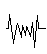
\includegraphics{figs/chapter2/mtt/wave.png}
    \caption{PhonR}
  \end{subfigure}
  \caption{語義-文字理論。}
  \label{fig:mtt}
\end{figure}
句法(syntax)可定義為支配句子結構,決定詞、子句如何組成其上級結構的一系列規則。
根據梅氏(Igor Mel’čuk)的文字-語意理論(Meaning-text theory, 見圖\ref{fig:mtt}),
一段語句的生成可以被描述為從語意表徵(semantic representation, SemR)到語音表徵(phonetic representation, PhonR)之間一連串的轉換(見圖n):
語意表徵先經由一普遍適用的語法規則產生其深層語法表徵(deep syntactic representation, DSyntR),
爾後經由各語言的語法規則(syntactic rules)轉換為該語言特有的表層語法表徵(surface syntactic representation, SSyntR);
接著再透過各語言的線性化(linearization)規則轉換為構詞表徵(morphological representation, MorphR);最後轉化為語音表徵,成為一般人所聽見的語句。
從語意到語音的映射為一多對多的函數:同樣的語意可以用不同詞彙及語法結構表示(一對多),即改述(paraphrasing);
不同語意表徵的語句亦有可能經轉換後恰巧有相同的語音表徵(多對一),如圖\ref{fig:struct-ambig},英文語句``I saw a man with a telescope.'',
兩種不同語意表徵的語句(「我看見一個帶望遠鏡的男人」與「我用望遠鏡看見一個男人」)分別產生不同的語法表徵,最後因英文的線性化規則恰巧產生相同的語音表徵。
此示例說明了句法剖析對於語意理解的重要性:同樣的一句話可能根據不同的句法結構導出不一樣的語意。

\begin{figure}[tbp]
\centering
\begin{subfigure}[b]{1.\textwidth}
  \centering
  \captionsetup{justification=centering}
  \begin{dependency}[edge style={black!60!black,very thick},
    label style={fill=yellow!60,font=\bfseries,thick}]
    \begin{deptext}[column sep=0.3cm, row sep=0.5ex, font=\rmfamily]
      PROPN\& VERB\& DET\& NOUN\&  ADP\& DET\&      NOUN\& PUNCT \\
      I\&     saw\&    a\&  man\& with\&   a\& telescope\&   .\& \\
    \end{deptext}
  \depedge{2}{1}{nsubj}
  \deproot[edge unit distance=4ex]{2}{root}
  \depedge{4}{3}{det}
  \depedge{2}{4}{obj}
  \depedge{7}{5}{case}
  \depedge{7}{6}{det}
  \depedge{4}{7}{nmod}
  \depedge[edge unit distance=2ex]{2}{8}{punct}
  \wordgroup[group style={fill=gray!40, draw=brown, inner sep=.6ex}]{2}{1}{1}{a0}
  \wordgroup[group style={fill=orange!40, draw=brown, inner sep=.6ex}]{2}{2}{2}{a1}
  \wordgroup[group style={fill=blue!40, draw=brown, inner sep=.6ex}]{2}{3}{7}{a2}
  \end{dependency}
  \caption{介系詞片語``with a telescope''依附於名詞``a man''上;\\翻譯:我看見一個帶望遠鏡的男人。}
  \label{fig:np-attach}
\end{subfigure}
\vfill
\begin{subfigure}[b]{1.\textwidth}
  \centering
  \begin{dependency}[edge style={black!60!black,very thick},
    label style={fill=yellow!60,font=\bfseries,thick}]
    \begin{deptext}[column sep=0.3cm, row sep=0.5ex, font=\rmfamily]
      PROPN\& VERB\& DET\& NOUN\&  ADP\& DET\&      NOUN\& PUNCT \\
      I\&     saw\&    a\&  man\& with\&   a\& telescope\&   .\& \\
    \end{deptext}
  \depedge{2}{1}{nsubj}
  \deproot[edge unit distance=4ex]{2}{root}
  \depedge{4}{3}{det}
  \depedge{2}{4}{obj}
  \depedge{7}{5}{case}
  \depedge{7}{6}{det}
  \depedge[edge unit distance=1.75ex]{2}{7}{obl}
  \depedge[edge unit distance=1.75ex]{2}{8}{punct}
  \wordgroup[group style={fill=gray!40, draw=brown, inner sep=.6ex}]{2}{1}{1}{a0}
  \wordgroup[group style={fill=orange!40, draw=brown, inner sep=.6ex}]{2}{2}{2}{a1}
  \wordgroup[group style={fill=blue!40, draw=brown, inner sep=.6ex}]{2}{3}{4}{a2}
  \wordgroup[group style={fill=orange!40, draw=brown, inner sep=.6ex}]{2}{5}{7}{a1}
  \end{dependency}
  \caption{介系詞片語``with a telescope''依附於動詞``saw''上。\\
           翻譯:我用望遠鏡看見一個男人。}
  \label{fig:vp-attach}
\end{subfigure}
\caption{介系詞片語依附(Prepositional phrase attachment, PP attachment)造成的結構歧義性(Structural ambiguity)。}
\label{fig:struct-ambig}
\end{figure}
\begin{figure}
  \centering
  \begin{subfigure}[b]{.49\textwidth}
    \centering
    \begin{tikzpicture}
        \Tree 
        [.S [.NP [.N I ] ]
        [.VP [.V saw ]
        [.NP [.NP [.Det a ] [.N  man ]]
            [.PP [.P with ] [.NP [.Det a ] [.N telescope ]]]]
        ]]
    \end{tikzpicture}
    \caption{圖\ref{fig:np-attach}的成分句法剖析}
  \end{subfigure}
  \begin{subfigure}[b]{.49\textwidth}
    \centering
    \begin{tikzpicture}
        \Tree 
        [.S [.NP [.N I ] ]
        [.VP [.V saw ]
        [.NP [.Det a ] [.N  man ]]
        [.PP [.P with ] [.NP [.Det a ] [.N telescope ]]]]
        ]]
    \end{tikzpicture}
    \caption{圖\ref{fig:vp-attach}的成分句法剖析}
  \end{subfigure}
\end{figure}
%\begin{figure}
%\begin{figure}
\begin{dependency}
    \begin{deptext}
        DET \& NOUN \& AUX \& ADJ \& AUX \& PUNCT \\
        Der \& Blattrand \& kann \& bewimpert \& sein \& . \\
        \end{deptext}
        \depedge{2}{1}{det}
        \depedge{4}{2}{nsubj}
        \depedge{5}{3}{aux}
        \deproot{4}{root}
        \depedge{4}{5}{cop}
        \depedge{4}{6}{punct}
\end{dependency}
%\end{figure}
\end{figure}


依存句法(dependency grammar)則為句法理論的一支,將句法結構視為詞與詞之間的相依關係,以有向鏈結(directed links)將詞關聯在一起;
相較於成分句法(constituency grammar)只能表示連續結構(continuous constituents),當遇到不連續結構時只能以最相近的連續結構近似,
依存句法則無此限制,因此特別適合分析語序相對自由的語言。

\subsection{定義及問題描述}
給定一句話$\MSent = (\MWord_{1}, \MWord_{2}, \ldots, \MWord_{N})$,$\MWord_{n}$代表一個詞(word),
該句裡所有詞的集合$\MWords = \left.\{\MWord_{i}\}\right\vert_{i=1}^{N}$。
以詞 $\MWord \in \MWords$ 為節點,
,及詞之間所有可能的邊
$\mathcal{\MDepRels} = \{(\MWord_{i}, \MWord_{j})\ |\ \MWord_{i},\MWord_{j} \in \MWords, \MWord_{i} \neq \MWord_{j}\}$:
%句法關係 $\MDepRel = (\MWord_{i}, \MWord_{j}) \in \MDepRels$ 為詞$\MWord$之間的(有向)邊,
依存句法樹為一單一根有向樹(single-rooted arborescence)$\MTree=(\MWords, \MDepRels),\ \MDepRels \subset \mathcal{\MDepRels}$,
亦即其為一滿足以下限制的有向圖:
\begin{itemize}
    \item 整個有向圖只有一個根節點(root,無入邊的節點)。
    \item 除了根節點以外,每個節點皆有剛好一條入邊。
    \item 每個節點都存在剛好一條路徑從根節點到該節點。
\end{itemize}

因此給定句子$\MSent$,其所有合法單一根有向樹集合$\MakeUppercase{\MTree}(\MSent)$,
一剖析器$\MSent \mapsto \MTree,\ \MTree \in \MakeUppercase{\MTree}(\MSent)$,
其目標便是從所有可能的樹集$\MakeUppercase{\MTree}(\MSent)$中找出一顆樹$\MTree'$,
使得其與正確的樹$\MTree^{*}$之差異愈小愈好。

\subsubsection{依存關係之標籤}
在依存句法樹裡,每個依存關係$r$都會有其標籤$l$描述該依存關係的性質,
而剖析器給定句子$\MSent$預測完依存關係$R$後也需要正確預測每個依存關係$r \in R$的標籤$l$。
%令標籤集為$\mathcal{L}$,定義關係到標籤的映射$\ell: R \rightarrow \mathcal{L}$。
不同語言的句法有許多相同與不同之處,
為了求同存異,
UD句法樹庫在句法關係的分類上採取兩階層的架構,
在第一個階層定義了37種所有語言共享的普適句法關係(universal syntactic relations),
每個語言原本定義的各種語言專屬的句法關係都會被歸類到第一層的普適句法關係中的某一種關係,
而語言內的句法關係若需要更細緻的分類,
則可以放進第二層的語言專屬關係(language specific relations),
標籤的形式為$\textrm{普適句法關係}:\textrm{語言專屬關係}$。

\subsubsection{評估指標(evaluation metric)}

現行評斷依存句法剖析器輸出好壞的數值為標籤不計依附分數(Unlabeled Attachment Score, UAS)與標籤依附分數(Labeled Attachment Score, LAS)。
由於句法剖析樹每個詞都有父節點(除了根節點以外)的特性,
依附分數利用此性質,以詞為單位,計算剖析器成功預測每個詞的父節點詞的比例:
\begin{equation}
    \textrm{標籤不計依附分數} = \frac{\#\textrm{父節點詞與正確答案相同的詞}}{\#\textrm{詞}} \textrm{。}
\end{equation}
而沒有父節點詞的根節點詞,剖析器則要正確判斷其沒有父節點詞。

標籤依附分數則計算父節點詞與通往父節點的邊其依存關係標籤兩者均預測正確的比例:
\begin{equation}
    \textrm{標籤依附分數} = \frac{\#\textrm{父節點詞、依存關係標籤與正確答案相同的詞}}{\#\textrm{詞}} \textrm{。}
\end{equation}

\begin{table}[h!]
    \centering
    \begin{tabular}[t]{|l | l l|}
        \hline
        \textbf{句法關係} & \textbf{英文描述} & \textbf{中文描述} \\
        \hline
        \texttt{acl} & clausal modifier of noun (adjectival clause) & 形容詞子句 \\
        \texttt{advcl} & adverbial clause modifier & 副詞子句 \\
        \texttt{advmod} & adverbial modifier & 副詞 \\
        \texttt{amod} & adjectival modifier & 形容詞 \\
        \texttt{appos} &  appositional modifier & 同位語 \\
        \texttt{aux} & auxiliary & 助動詞 \\
        \texttt{case} & case marking & 格位 \\
        \texttt{cc} &  coordinating conjunction & 並列連詞 \\
        \texttt{ccomp} & clausal complement & 子句補語 \\
        \texttt{clf} & classifier & 分類詞 \\
        \texttt{compound} & compound & 複合(名詞、動詞等)\\
        \texttt{conj} & conjunct & 並列 \\
        \texttt{cop} & copula & 系詞 \\
        \texttt{csubj} & clausal subject & 子句主詞 \\
        \texttt{dep} & unspecified dependency & 未定義依存關係 \\
        \texttt{determiner} & determiner& 限定詞 \\
        \texttt{discourse} & discourse element & 話語元素 \\
        \texttt{dislocated} & dislocated elements & 錯位 \\
        \texttt{expl} & expletive & 虛主詞 \\
        \texttt{fixed} & fixed multiword expression & 固定多詞表達 \\
        \texttt{flat} & flat multiword expression & 扁平多詞表達 \\
        \texttt{goeswith} & goes with & 同詞 \\
        \texttt{iobj} & indirect object & 間接受詞 \\
        \texttt{list} & list & 列舉 \\
        \texttt{marker} & marker & 標記 \\
        \texttt{nmod} & nominal modifier & 名詞修飾語 \\
        \texttt{nsubj} & nominal subject & 名詞主語 \\
        \texttt{nummod} & numeric modifier & 數值修飾語 \\
        \texttt{obj} & object & 受詞 \\
        \texttt{obl} & oblique nominal & 間接格名詞 \\
        \texttt{orphan} & orphan & 孤懸 \\
        \texttt{parataxis} & parataxis & (句子)並列 \\
        \texttt{punct} & punctuation & 標點 \\
        \texttt{reparandum} & overridden disfluency & 修護語 \\
        \texttt{root} & root & 根 \\
        \texttt{vocative} & vocative & 呼格 \\
        \texttt{xcomp} & open clausal complement & 開放子句補語 \\
        \hline
    \end{tabular}
    \caption{UD句法樹庫裡的普適句法關係。}
    \label{tab:deprels}
    \end{table}
%剖析器除了要正確判斷依存關係$R$之外,
%但由於依存句法樹作為根節點的詞沒有父節點,
%為了有利讓根節點的每個詞都有父節點,我們可以新增一個節點作為這顆樹新的根節點,讓原本作為根節點的詞的父節點指向該新的根節點。
%其中每個剖析器對該差異函數$L$之定義均有不同;下節會給出圖類剖析器對$L$的常見定義。

%以圖的觀點視之,則節點nodes,vertices)為詞(words)、相依關係為邊(edge)
\subsection{圖類剖析器 (Graph-based Parser)}
\label{subsec:graph_parser}

圖類剖析器的運作方式簡介如下:
圖類剖析器為所有合法的單一根有向樹進行評分,其方式為將每顆樹 $\MTree = (W, R)$ 的分數拆分成其所有組成邊的分數之加總:
\begin{equation}
    \TreeScore (\MTree) = \exp{ \left( \sum_{r \in R} \MScore(\MDepRel) \right) }
\end{equation}
其中 $\TreeScore(\MTree)$ 為樹 $\MTree$ 的評分函數,$\MScore(r)$為邊$\MDepRel$的評分函數。

而最佳的生成有向樹 $\MTree^{*}$ 就是分數最高的生成有向樹:
\begin{equation}
    \MTree^{*} = \argmax_{\MTree}\ \TreeScore (\MTree) = \argmax_{\MTree = (W, R) \in \MakeUppercase{\MTree}(\MSent)}\ \exp{ \left( \sum_{r \in R} \MScore(\MDepRel) \right) }
\end{equation}
上述最佳生成有向樹 $\MTree^{*}$ 可由執行最大生成有向樹演算法(maximum-spanning aborescence algorithm,見演算法\ref{alg:cle})得出。
因此圖類剖析器旨在學習一個評分函數 $\MScore((\MWord_{i}, \MWord_{j}))$ ,使得給定訓練資料裡的樹$G=(V, E)$,
使得正確句法樹中的邊 $(\MWord_{i}, \MWord_{j}) \in E$ 其分數 $\MScore((\MWord_{i}, \MWord_{j}))$ 被拉高,
其餘沒有出現在句法樹中的邊 $(\MWord_{i}, \MWord_{j'}) \notin E$ 其分數 $\MScore((\MWord_{i}, \MWord_{j'}))$ 被拉低。

\subsubsection{全域似然性(global likelihood)}

為了拉高正確句法樹的分數與拉低錯誤句法樹的分數,給定參數$\theta$的剖析器機率函數
$p_{\theta} (\MTree|\MSent): \MakeUppercase{\MTree}(\MSent) \rightarrow [0, 1]$,
我們可以定義句法樹的模型機率為該句法樹的分數除以所有可能句法樹集合$\MakeUppercase{\MTree}$的分數總和:
\begin{equation}
    p_{\theta} (\MTree) = \frac{\TreeScore(\MTree)}{\sum\limits_{\MTree' \in \MakeUppercase{\MTree}}  \TreeScore(\MTree')}\textrm{。}
\end{equation}
其中分母又稱為句法樹的配分函數(partition function)。
分母的配分函數看似難以計算,幸虧所有可能句法樹的分數總和可以透過克氏矩陣-樹定理( Kirchhoff’s Matrix-Tree Theorem)快速計算出來\cite{Tutte1984GraphT}。
因此我們只要優化正確句法樹的機率$p_{\theta} (\MTree)$,正確句法樹的分數與錯誤句法樹的分數自然會分別被拉高與拉低。
2007年的古氏(Terry Koo)\cite{koo-etal-2007-structured}與2017年的馬氏(Xuezhe Ma)\cite{ma-hovy-2017-neural}
均採用該定理有效率地計算配分函數。

\subsubsection{父節點選擇交叉熵(headword selection cross-entropy)}

相較於上節使用矩陣-樹定理得出精確的句法樹機率,多氏\cite{Dozat2017DeepBA}在該篇論文中採用較為簡單的演算法近似句法樹機率;
如前述,由於句子中的每個詞都剛好需要從其他詞中選擇一詞作為其父節點詞(或者指定該詞為「根」),
令$h(w)$為詞$w$的父節點,
$W^{+} = W + \{\texttt{root}\}$($(\texttt{root}, w)$代表$w$為根節點),
他將句法樹的機率用每個詞選擇其父節點詞的機率相乘來代表:
\begin{equation}
    p_{\theta} (\MTree) = \prod_{w \in W} \frac{e^{\MScore((h(w), w))} }{\sum\limits_{w' \in W^{+}, w' \neq w} e^{\MScore((w', w))}}
    \textrm{。}
\end{equation}

\begin{algorithm}
    \begin{spacing}{1.0}
        \begin{algorithmic}
            \Procedure{\textbf{最大生成有向樹}}{$G,s$}
            \State $G = \left(V,\ E\right)$
            \State 邊評分函數 $s: E \rightarrow \mathbb{R} $
            \State $E' = \{\left(\MWord_{i}, \MWord_{j}\right)| \MWord_{j} \in V, \MWord_{i} = \underset{\MWord_{i}}{\argmax}\ s\left(\MWord_{i}, \MWord_{j}\right)\}$
            \State $G' = \left(V, E'\right)$
            \If{$G'$ 無環}
                \State{回傳 $G'$}
            \Else
                \State 尋找一邊集合 $E_{C}$ 使得其為 $G'$ 中的環
                \State $G_{C} = \textbf{收束}\left(G', E_{C}, s\right)$
                \State $\mathbf{y} = \textbf{最大生成有向樹}\left(G_{C}, s\right)$
                \State 尋找一節點 $v \in C$ 使得 $(v', v) \in \mathbf{y}, (v'', v) \in C$
                \State 回傳 $\mathbf{y} \cup C - \{(v'', v)\}$
            \EndIf
            \EndProcedure
            \Procedure{\textbf{收束}}{$G, E_{C}, s$}
                \State 令 $G_{C}$ 為 $G$ 除去 $C$ 中的節點後的子圖
                \State 將 節點 $c$ 加入 $G_{C}$ 中,代表原本的環 $C$
                \For{$v \in V - C: \exists_{v' \in C}\ (v', v) \in E$}
                    \State 將邊 $(c, v)$ 加入 $G_{C}$, 其分數 $s(c, v) = \max_{v' \in C} s(v', v)$
                \EndFor
                \For{$v \in V - C: \exists_{v' \in C}\ (v, v') \in E$}
                    \State 將邊 $(v, c)$ 加入 $G_{C}$, \par
                    \hskip\algorithmicindent $s(v, c) = \max_{v' \in C} \left[s(v, v') - s(a(v'), v') + s(C)\right]$, \par
                    \hskip\algorithmicindent $a(v)$ 為 $v$ 之父節點 $C$, \par
                    \hskip\algorithmicindent $s(C) = \sum_{v \in C} s(a(v), v)$
                \EndFor
                \State 回傳 $G_{C}$
            \EndProcedure
        \end{algorithmic}
        \caption{最大有向樹演算法。}
        \label{alg:cle}
    \end{spacing}
\end{algorithm}
\section{基於優化的元學習 (Optimization-based Meta Learning)}
\label{sec:mamls}
\subsection{模型無關元學習 (Model-agnostic Meta Learning, MAML)}
模型無關元學習於2017年由芬氏(Chelsea Finn)提出,為基於優化的元學習方法的一種,
將元學習的宗旨「學習如何學習」(learning to learn)理解為對某些任務學習一個好的初始模型參數,
使得模型在碰到新任務時能夠學得更快更好。

現在我們將上面的敘述改寫為數學語言:
給定一任務分佈$\mathcal{T}$、
從任務分佈中採樣出的任務$\tau \sim \mathcal{T}$、
每個任務對應的訓練損失函數 $\mathcal{L}_{\tau,A}$ 與測試損失函數 $\mathcal{L}_{\tau,B}$ 、
模型無關元學習目標是找尋一參數$\phi$,使得參數在任務分佈下採樣出的每個任務,用訓練資料分別進行$k$次更新後的參數(此步驟稱為內循環,inner-loop),
在各自任務上的測試損失函數最小:
\begin{align}
    \phi^{\ast} = \argmin_{\phi} \mathbb{E}_{\tau \sim \mathcal{T}} \left[ \mathcal{L}_{\tau,B} \left( U_{\tau,A}^{k} (\phi) \right) \right] \label{eq:maml}\\
    U_{\tau}^{k} \left( \phi \right) = \underbrace{U_{\tau} ( ... U_{\tau} ( U_{\tau} }_{\texttt{k times}} ( \phi ) ) ... )
\end{align}
其中更新函數$U_{\tau}(\phi)$可以用任何優化器實現,比如陽春SGD(Vanilla SGD):
\begin{equation}
U_{\tau, \textrm{SGD}} \left( \phi \right) = \phi - \alpha \nabla_{\phi} \mathcal{L}_{\tau} \left( \phi \right)
\end{equation}
或者Adam優化器$U_{\tau,\textrm{ADAM}}(\phi)$\cite{kingma2014adam}。
模型無關元學習針對式\ref{eq:maml}的解法是再做一次梯度下降法(此步驟稱為外循環,outer-loop):
\begin{align}
    g_{\mathrm{MAML}} &= \frac{\partial }{\partial \phi} \mathcal{L}_{\tau, B} \left( U_{\tau, A} (\phi) \right) \\
                      &= U'_{\tau, A} (\phi) \mathcal{L'}_{\tau, B} ( \widetilde{\phi} ),\quad \text{其中}\quad \widetilde{\phi} = U_{\tau, A} (\phi) \label{eq:gradmaml}
\end{align}
式\ref{eq:gradmaml}的 $U'_{\tau, A} (\phi)$為更新函數$U_{\tau, A}$的雅可比矩陣(Jacobian Matrix),含有參數的二階導數。
下以陽春SGD為例,推導為何上式有二階導數:

令初始參數為$\phi_{0}$,更新$k$次後的參數為$\phi_{k}$,則更新$k$次的函數的導數(以下省略$A$)$\left( U_{\tau}^{k} \right)' \left(\phi_{0}\right)$可以寫成:
\begin{align}
    \left( U_{\tau}^{k} \right)' \left(\phi_{0}\right) &= \frac{\partial \phi_{k}}{\partial \phi_{0}} \\
                                                       &= \prod\limits_{i=0}^{k-1} \frac{\partial \phi_{i+1}}{\partial \phi_{i}} 
\end{align}
我們將單步更新的導數寫出來:
\begin{align}
    \frac{\partial \phi_{i+1}}{\partial \phi_{i}} &= \frac{\partial}{\partial \phi_{k}} \left( \phi_{k} - \alpha \nabla_{\phi_{k}} \mathcal{L}_{\tau} \left( \phi_{k} \right) \right) \\
                                                  &= I - \alpha \nabla^{2}_{\phi_{k}} \mathcal{L}_{\tau} \left( \phi_{k} \right)
\end{align}
因此$k$步更新的導數可以寫成單步更新參數之黑塞矩陣(Hessian)的連乘:
\begin{equation}
    \left( U_{\tau}^{k} \right)' \left(\phi_{0}\right) = \prod\limits_{i=0}^{k-1}  \left( I - \alpha \nabla^{2}_{\phi_{i}} \mathcal{L}_{\tau} \left( \phi_{i} \right) \right)
\end{equation}
代入式\ref{eq:maml}後,我們得到
\begin{align}
    g_{\mathrm{MAML}}^{k} &= \left(U_{\tau, A}^{k}\right)' (\phi) \mathcal{L'}_{\tau, B} ( \widetilde{\phi} ) \\
                      &= \mathcal{L'}_{\tau, B} ( \phi_{k} ) \prod\limits_{i=0}^{k-1}  \left( I - \alpha \nabla^{2}_{\phi_{i}} \mathcal{L}_{\tau, A} \left( \phi_{i} \right) \right) \\
                      &= \nabla_{\phi_{k}} \mathcal{L}_{\tau, B} ( \phi_{k} ) \prod\limits_{i=0}^{k-1}  \left( I - \alpha \nabla^{2}_{\phi_{i}} \mathcal{L}_{\tau, A} \left( \phi_{i} \right) \right)
\end{align}
由於模型的參數維度非常大,計算其黑塞矩陣需要耗費大量計算資源,因此之後的研究者紛紛對模型無關元學習提出不需要計算黑塞矩陣的一階近似元學習方法。
以下介紹\fomaml(First-order MAML)與\reptile (Reptile)\cite{nichol2018first}兩種變形。
\subsection{\fomaml (First-order MAML)}
\fomaml法直接將原本模型無關元學習之更新函數的導數$\left(U_{\tau, A}^{k}\right)' (\phi)$設為單位矩陣:
\begin{align}
    g_{\mathrm{FOMAML}}^{k} &= g_{\mathrm{MAML}}^{k}\bigg|_{\left(U_{\tau, A}^{k}\right)' (\phi) = I} \\
    &= \mathcal{L'}_{\tau, B} (\phi_{k} )
\end{align}
\subsection{\reptile (Reptile)}
\reptile直接將其梯度設爲各個任務參數更新前後差值$\phi - U_{\tau_{A}}^{k}(\phi)$的平均:
\begin{align}
    g_{\mathrm{REP}}^{k} &= \mathbb{E}_{\tau}\left[ \left( \phi - U_{\tau_{A}}^{k}(\phi) \right) \right]
\end{align}
當$k = 1$時,此演算法與普通的多工訓練(multi-task training)並無二致。但當$k > 1$時,此更新含有$L_{\tau_{A}}$的高次導數,
使得其行為與多工訓練多所不同。

\iffalse
\section{模型內插法(Model Interpolation)}

雖然類神經網路在影像、語言及語音均取得巨大的成功,優化過後的網路其內部運作機制卻宛如黑箱般難以被解釋。
這樣的現象可能阻礙類神經網路的發展,因為研究者無法透過分析模型的運作機制來改進模型架構;
因此許多研究者開始發展分析類神經網路的方法,
而模型內插法為其中一種分析模型的技巧,初見於2015年谷氏等人\cite{Goodfellow2015QualitativelyCN}對類神經網路的分析。
模型內插法直接在有興趣的模型之間(或附近)可視化一般認為極度非convex(highly non-convex)的損失平面。

\subsection{線性內插(Linear Interpolation,Lerp)}
給定有興趣分析的兩個模型及其參數$\phi_{1}$、$\phi_{2}$,線性內插法直接在通過這兩個參數的射線上計算在該點的損失:
\begin{equation}
    \mathbf{Lerp} \left( \phi_{1}, \phi_{2} ; \alpha \right) = \alpha \phi_{1} + (1 - \alpha) \phi_{2},\ \alpha \in \mathbb{R}.
\end{equation}
\subsection{球面線性內插(Spherical Linear Interpolation,Slerp)}
給定有興趣分析的兩個模型及其參數$\phi_{1}$、$\phi_{2}$,球面線性內插法可以被視為線性內插法的球面版本:
\begin{align}
    \mathbf{Slerp} \left( \phi_{1}, \phi_{2} ; \alpha \right) &= \frac{\sin [\alpha\Omega]}{\sin \Omega} \phi_{1} + \frac{\sin [(1-\alpha) \Omega]}{\sin \Omega} \phi_{2},\ \alpha \in \mathbb{R}. \\
    \Omega &= \cos^{-1} \left( \frac{\phi_{1} \cdot \phi_{2}}{ \left\lVert \phi_{1} \right\rVert \cdot \left\lVert \phi_{2} \right\rVert} \right)
\end{align}
\fi
\chapter{實驗A}
  \section{簡介}
%文獻上已經提出許多改進資料不足語言的句法剖析的方法,其中多半需要該資料不足語言的特性,用以找尋與其相似的語言進行協同訓練。
%近年來初見於影像領域的模型無關元學習,本來是為了處理少量樣本學習的問題,
%不久後也為資料不足(但資料量大於少量樣本學習)的學習任務所用\cite{gu-etal-2018-meta},
%不需要事先知道任務的特性,

\iffalse
有名的語言學家杭氏(Noam Chomsky)觀察人類習得語言的過程,
他認為嬰孩學習語言時所接收到的語言輸入是不足以讓他們習得該語言的所有特徵的,
許多特性相異的語法都可以產生這些他們所接收到的語料,
但孩童仍然習得了該語言的正確語法,
因此他推斷人類出生時大腦中即具備有某種語言習得裝置(Language acquisition device),
而語言習得裝置的任務便是從所有與語料匹配的語法中挑選正確的語法
\fi
本章介紹使用模型無關元學習進行多語言預訓練,以幫助資料不足語言的依存句法剖析的系列實驗。

模型無關元學習本來是為了處理圖片分類領域少量樣本學習的問題,
不久後也為資料不足(但資料量大於少量樣本學習)的學習任務所用,
如古氏(Jiatao Gu)將元學習方法引入資料不足的機器翻譯,
並勝過使用普通多語言學習的基準模型\cite{gu-etal-2018-meta}。
芬氏(Chelsea Finn)在2018年提出的模型無關元學習(model-agnostic meta-learning)
\cite{Finn2017ModelAgnosticMF}為所有使用梯度下降法(gradient descent)進行最佳化的模型提供了一項簡潔且有效的方法處理資料不足任務。
在語言轉移學習的框架下,其目標是替未見過的語言(unseen languages)尋找一合適參數初始值,使得少量步數梯度更新後,參數在該語言的測試集上表現最佳,
其稱此在少量步數更新就能大幅增進爲見過語言表現的能力為「快速適應」(fast adaptation)\cite{Finn2017ModelAgnosticMF}。
%其強調使用少量步數進行梯度更新,即是由於資料不足語言資料稀少,過多步數容易過擬合。

在元學習出現以前,
若希望利用相似語言中所蘊含的資訊給予模型語言普遍具備的歸納偏置(下稱普適語言偏置,universal linguistic biases),
多語言學習(multilingual learning)為一主要的方法\cite{caruana1997multitask}。
藉由共享特徵抽取網路並用以同時訓練多種相關語言,
相關語言的資訊得以透過反向傳播(backpropagation)注入類神經網路中,
使模型相較於解釋單一語言,更加偏好能夠解釋所有相關語言的假說,
有效幫助模型達成泛化(generalization)。

然而多語言訓練的目標,是提高訓練語言(training languages)在其測試集(testing set)上的準確率,
而提高訓練語言的準確率,未必就代表在資料不足語言上的準確率也會隨之提高;
有可能出現訓練語言與資料不足語言差異過大,而導致多語言訓練模型無法幫助資料不足語言的任務表現。

不若單純的多語言訓練,模型無關元學習於訓練階段的目標並非提高在訓練語言上的表現,
而是直接最佳化模型在未見過語言上\finetune 後的表現,訓練與測試環境沒有不匹配之處,
有效防止模型只在訓練語言的測試集上有好表現,而無法推廣到資料不足語言上的問題。

\iffalse
尤其當目標任務缺乏資料的時候,若使用過於有表現力的假說集合,
易使模型過擬合到目標任務上,
利用相似任務進行多工學習幫助目標任務提升表現的效果尤其顯著。
然而多工學習得到的模型可以在訓練過的所有任務上的測試集有好表現,
但並未保證這樣的好表現可以轉移到相似但未見過的任務上;
而芬氏(Chelsea Finn)提出的模型無關元學習(model-agnostic meta-learning)
\cite{Finn2017ModelAgnosticMF}提供了多工學習之外的另一種方法,
將領域的歸納偏置(inductive bias)注入類神經網路中。
\fi

%\section{相關研究}


\section{多語言去詞化依存句法分析(multilingual delexicalized dependency parsing)}
由於詞化的依存句法分析有太多變因,包括使用的預訓練模型,其對不同語言的偏置等等,都會影響句法剖析模型於目標語言上的行為;
且詞化的依存句法分析參數量較多,使用二次微分的計算量與佔用空間均較大,訓練耗時,
有時甚至會發生用來進行平行矩陣運算的圖形處理器記憶體不足的問題。
因此為了排除語言本身句法以外性質對句法剖析的影響及計算資源的考量,
本節先進行去詞化依存句法分析的實驗,
也就是只使用句法樹庫提供的詞性標記做為詞的表徵進行句法剖析。

\subsection{詞性標記(POS tags)}
UD句法樹庫中大部分的語言均提供兩種詞性標記:專為該語言設計的詞性標記(XPOS),通常為該句法樹庫尚未整合進UD時原本的詞性標記,
與各語言統一的普適詞性標記\cite{petrov-etal-2012-universal}(Universal POS tags, UPOS),
其捨棄各語言細緻的詞性分別,
整合語言間相似性質的詞性,以達到所有語言共享同一組詞性集合的目標。
如前置介系詞(prepositions)與後置介系詞(postpositions)在UPOS的框架下就被整合成介系詞(adpositions)而不做前後置之分。
由於UPOS有更好的跨語言通用性,本研究去詞化句法剖析的詞性標記輸入均使用UPOS。

\subsection{修訂版爬蟲類元學習}
原始版本的爬蟲類元學習\cite{nichol2018first}無論是在內循環或外循環的開頭都不會重新啟動內循環的優化器,
當使用有動能(momentum)的優化器如Adam時,當下的梯度更新會受之前用其他語言計算而得的梯度影響,
造成語言間不必要的干擾。
為了避免此現象,原作者將一階動能項$\beta_{1}$設為$0$。
%然而mBERT原始論文中進行精細校正使用的為具有動能項的Adam,
然而本研究的初始實驗發現$\beta_{1} = 0$的Adam在精細校正時時會對準確率造成負面影響。
再者,爬蟲類元學習將外循環原始梯度(raw gradient)直接設為各語言內循環(亦即精細校正)前後參數的差異的平均,
此數值大小很大程度上取決於內循環優化器的學習率,
恐與一般模型精細校正時接收到的梯度分佈差異過大。

為處理此問題,本研究稍稍修改了爬蟲類元學習的演算法,
希望在不改變內循環優化器設置的前提下保留爬蟲類元學習加總內循環所有梯度的優點:
與其將內循環梯度設為前後參數的差異的平均 $\phi - U_{\textrm{ADAM}}^{k}(\phi) $,
內循環原始梯度經過內循環優化器處理過後的產物,
本研究將內循環梯度直接設為內循環\textbf{原始}梯度的平均(此處優化器以Adam為例):
\begin{equation}
    g_{\textrm{REP}} = \mathbb{E}_{\tau}\left[ \frac{1}{k} \sum_{i=1}^{k} \nabla_{\phi_{i}} \mathcal{L}_{\tau} \left( \phi_{i}^{\texttt{adam}} \right) \right]
\end{equation}
其中
\begin{equation}
    \phi_{i}^{\texttt{adam}} = U_{\textrm{ADAM}} \left( \phi_{i - 1}^{\texttt{adam}} \right).
\end{equation}
此數值雖然是由內循環優化器計算出來,但此處取其原始梯度,
受內循環學習率影響較小。
此修訂版爬蟲類元學習與普通的多語言學習的差異比起原始的爬蟲類元學習要來的更小:
外循環的梯度為內循環原始梯度的平均,與多語言學習類似;
但原始梯度仍是由內循環更新過的參數計算出來的(除了內循環的第一步),更接近原本的爬蟲類元學習。
初始實驗發現此修訂版爬蟲類元學習表現不俗,
且相較原始爬蟲類元學習的表現來的更加穩定。
往後提到的爬蟲類元學習均意指本節所提出的修訂版爬蟲類元學習。

\subsection{實驗設置}
\label{subsec:delex_depparse_setting}

\begin{table}[htbp]
    % \fontsize{8}{10}\selectfont
    \centering
    \begin{subtable}[t]{.4\textwidth}
        \begin{tabular}[t]{@{}lr@{}}
        \toprule
        超參數 & 值 \\
        \midrule
            詞性嵌入維度         & 100 \\
            編碼器              & 雙向LSTM \\
            編碼器層數           & 3 \\
            編碼器隱維度         & 100 \\
            依存標籤維度         & 200 \\
            依存邊維度           & 200 \\
            詞性丟棄機率            & 0.33 \\
            批次大小$b$         & 16 \\
            語言數$l$           & 10 \\
            訓練樣本數/回合        & 64000 \\
            訓練回合數          & 10 \\
            優化器              & Adam \\
            $\beta_1,\beta_2$  & 0.9, 0.9 \\
            權重衰減參數         & 0.01 \\
            基礎學習率          & $3e^{-4}$ \\
            最大梯度範數        & 5.0 \\
        \bottomrule
        \end{tabular}
        \caption{
            預訓練超參數。
        }
        \label{tab:delex_pretrain_hparams}
    \end{subtable}
    \begin{subtable}[t]{.4\textwidth}
        \begin{tabular}[t]{@{}lr@{}}
        \toprule
        超參數 & 值 \\
        \midrule
            優化器              & Adam \\
            基礎學習率          & $3e^{-4}$ \\
            $\beta_1,\beta_2$  & 0.9, 0.9 \\
            批次大小            & 16 \\
            訓練回合數          & 80 \\
            最大梯度範數        & 5.0 \\
            交叉驗證摺數$k$     & 3   \\
        \bottomrule
        \end{tabular}
        \caption{
            精細校正超參數。
        }
        \label{tab:delex_finetune_hparams}
    \end{subtable}
    \caption{
        模型超參數一覽。
    }
    \label{tab:delex_hparams}
\end{table}
我們從\conll 的53種訓練語言(73個訓練句法樹庫)中選取有官方驗證集(development set)的46種訓練語言(66個訓練句法樹庫)作爲訓練語言;見表\ref{tab:training_languages}。
預訓練完成後,我們分別對該模型進行\zeroshot 及\finetune 在預訓練中未見過的語言上。
我們挑選\conll 的訓練語言中剩下的只有訓練集而沒有發展集的語言作爲真實資料不足測試語言(true low-resource testing languages,見表\ref{tab:true_lr_testing_languages})。
為了觀察控制資料多寡時對不同預訓練方法的影響,
我們另外挑選了UD 2.5版中8種不在訓練語言中的語言做為模擬資料不足測試語言(simulated low-resource testing languages,見表\ref{tab:sim_lr_testing_languages})。
實驗在訓練與測試時時均使用正確的斷句、斷詞,並使用句法樹庫提供的正確詞性做為詞的表徵。

至於多語言訓練的部分,孔氏\cite{kondratyuk-straka-2019-75}與烏氏\cite{ustun2020udapter}進行多語言訓練的方法,
是將全部語言的句法樹庫接在一起、在一個小批次(batch)中混合多個句法樹庫訓練。
這樣的做法可能會導致資料量大的語言取樣頻率過高;
我們的方法則是每次更新從全部語言裡取樣$l$種語言,每種語言取樣$b$個句子,一個批次總共有$b \times l$個句子。
不同於孔氏與烏氏,這樣的方法防止模型過度對資料充足語言的特性建模,但也可能使得資料不足語言的句子被過度取樣而產生過擬合的現象。

超參數的設置見表\ref{tab:delex_hparams}。
\subsection{實驗結果}

\begin{figure}[htbp]
    \centering
    \begin{subfigure}[t]{\textwidth}
        \centering
        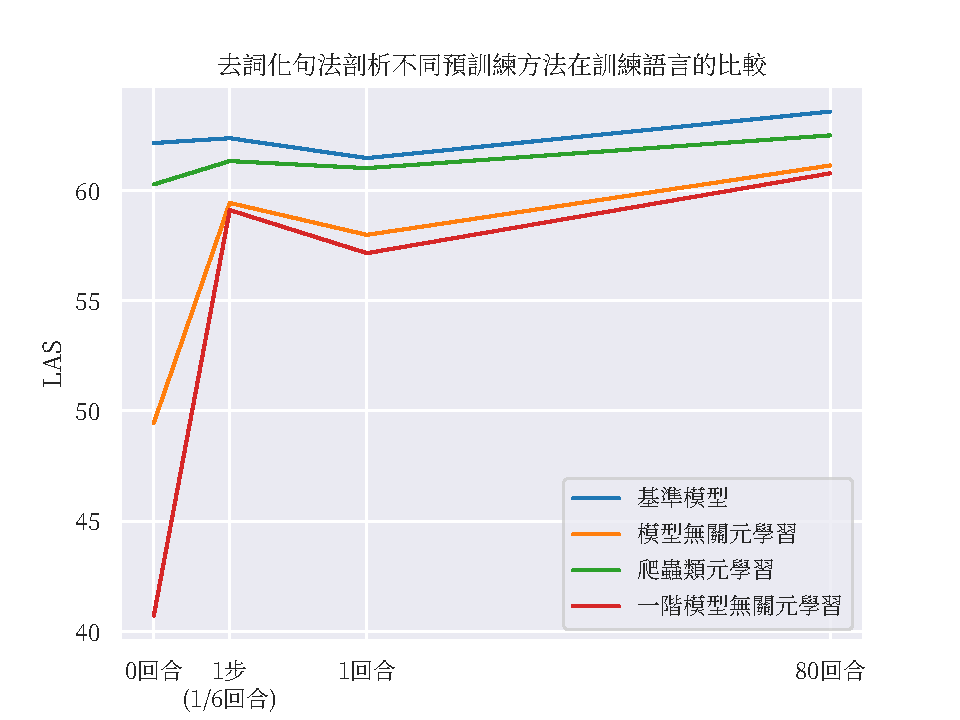
\includegraphics[width=\textwidth]{figs/chapter3/delex/delex_train_langs.pdf}
    \end{subfigure}
    \vspace{-12pt}
    \begin{subfigure}[t]{\textwidth}
        \centering
        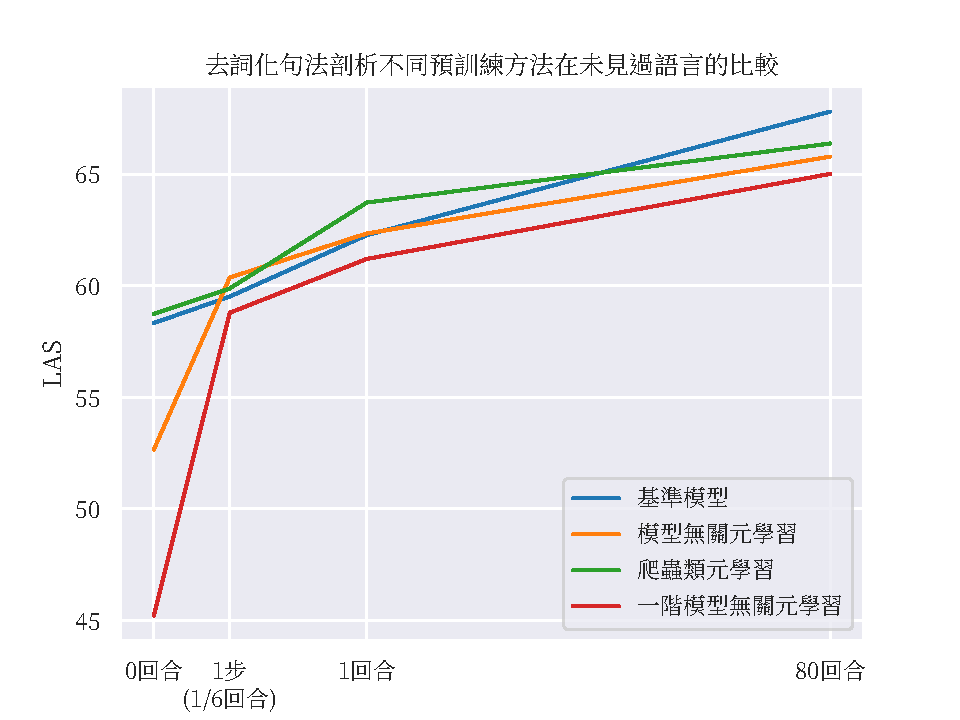
\includegraphics[width=\textwidth]{figs/chapter3/delex/delex_test_langs.pdf}
    \end{subfigure}
    \caption{去詞化分析不同預訓練方法精細校正後在測試集上的平均表現。}
    \label{fig:delex_avg}
\end{figure}
圖\ref{fig:delex_avg}為去詞化分析不同預訓練方法產生的模型在目標語言上經過不同步數的\finetune 後的測試集LAS數值。
由圖中可以觀察到:
\begin{itemize}
    \item 在未見過語言上,模型無關元學習模型於只精細校正一步的表現及相對於精細校正前的進步量均為各方法中之冠,
顯示模型無關元學習的確有快速適應的能力。
    %\item 在未見過語言上,模型無關元學習於
    \item 模型無關元學習模型在零樣本學習的表現大幅落後基準模型,說明其優勢主要在只需少量目標語言資料即可快速適應的能力,
    並不適合做為單一多語言模型同時處理多種語言。
    \item 在未見過語言上,\reptile 模型在零樣本學習、精細校正一步、一回合與八十回合的情況下表現均與基準模型不相上下,
在精細校正一步與一回合更稍稍勝過基準模型,顯示其適合用於剖析所有訓練與未見過的語言,又能夠受益於少量未見過語言的語料。
    \item 在所有語言上,無論接觸多少目標語言的語料(精細校正前、一步、一回合、八十回合),
\fomaml 模型均大幅落後其他所有模型,顯示只取內循環最後一步的梯度更新既不足以使模型學習到訓練語言的語法,
也無法泛化到未見過的語言上。
    \item 在訓練語言上,基準模型無論接觸多少目標語言的資料,其表現均大幅贏過模型無關元學習模型,
這說明基準模型的確達到其訓練目標-同時剖析所有的訓練語言。

    %\item 在訓練語言上在精細校正一步的設置中,模型無關元學習模型在訓練語言上以少量資料精細校正後,於測試集上的表現明顯不如基準模型,但在未見過語言以少量資料精細校正測試集上
\end{itemize}

以下為分語言、分接觸目標語言語料量的數據圖表。
%其中表\ref{tab:delex_las_epoch_1}
其中圖\ref{fig:bar_zs}、\ref{fig:bar_one_step}、\ref{fig:bar_full_epoch_1}、\ref{fig:bar_full_epoch_80}
為各方法接觸不同數量的各種目標語言的語料其表現的長條圖。
\iffalse
\begin{table}[htbp]
    \begin{subtable}[h]{0.8\textwidth}
        \centering
            \begin{tabular}[!ht]{c|llll}
                \hline
                語言 & 基準 & 模型無關元學習 & 爬蟲類元學習 & 一階模型無關元學習 \\
                \hline\hline
                wo & \textbf{62.83}** & 55.47 & \textbf{62.96}** & 45.69 \\
                gd & \textbf{44.47} & 37.42 & \textbf{44.14} & 34.97 \\
                te & 60.61 & 60.06 & \textbf{62.55} & 52.15 \\
                cop & \textbf{66.58} & 63.17 & \textbf{66.93} & 59.33 \\
                be & \textbf{71.87}** & 57.70 & 70.78 & 45.26 \\
                mr & \textbf{48.30}* & 42.48 & \textbf{47.33}* & 34.22 \\
                mt & \textbf{68.76}** & 61.77 & \textbf{68.42}** & 57.40 \\
                ta & 43.19 & 43.19 & \textbf{46.81}** & 32.73 \\
                \hline
                avg & 58.33 & 52.66 & \textbf{58.74} & 45.22 \\
                \hline
            \end{tabular}
            \caption{未精細校正(0回合)。}
    \end{subtable}
    \vfill
    \begin{subtable}[h]{0.8\textwidth}
        \centering
            \begin{tabular}[!ht]{c|llll}
                \hline
                語言 & 基準 & 模型無關元學習 & 爬蟲類元學習 & 一階模型無關元學習 \\
                \hline\hline
                wo & 63.64 & 63.91 & 63.39 & \textbf{64.22} \\
                gd & 46.49 & 45.87 & \textbf{47.96}* & 46.88 \\
                te & 64.36 & 65.05 & \textbf{65.60} & 62.55 \\
                cop & 67.03 & 66.99 & \textbf{67.44} & 66.93 \\
                be & \textbf{71.59}** & 69.13 & \textbf{71.11}** & 67.99 \\
                mr & 48.79 & \textbf{53.40}** & 47.57 & 48.54 \\
                mt & \textbf{68.84}* & 68.08 & \textbf{68.83}* & 68.04 \\
                ta & 45.35 & \textbf{50.48}** & 47.11 & 45.15 \\
                \hline
                avg & 59.51 & \textbf{60.36} & 59.88 & 58.79 \\
                \hline
            \end{tabular}
        \caption{精細校正1步($\frac{1}{6}$回合)。}
    \end{subtable}
    \vfill
    \begin{subtable}[h]{0.8\textwidth}
    \centering
        \begin{tabular}[!ht]{c|llll}
            \hline
            語言 & 基準 & 模型無關元學習 & 爬蟲類元學習 & 一階模型無關元學習 \\
            \hline\hline
            wo & 65.71 & 63.43 & \textbf{66.53}* & 61.40 \\
            gd & 53.79 & \textbf{57.30}** & \textbf{57.11}** & 55.74 \\
            te & 68.24 & 67.27 & \textbf{70.18} & 64.77 \\
            cop & 66.95 & 65.83 & \textbf{67.84}** & 64.86 \\
            be & \textbf{69.14}** & 65.57 & \textbf{69.51}** & 65.96 \\
            mr & 52.67 & \textbf{58.25} & 55.10 & 56.55 \\
            mt & \textbf{70.05}** & 67.33 & 69.20 & 66.83 \\
            ta & 51.58 & 53.75 & \textbf{54.35} & 53.49 \\
            \hline
            avg & 62.27 & 62.34 & \textbf{63.73} & 61.20 \\
            \hline
        \end{tabular}
        \caption{精細校正1回合。}
    \end{subtable}
    \vfill
    \begin{subtable}[h]{0.8\textwidth}
        \centering
            \begin{tabular}[!ht]{c|llll}
                \hline
                語言 & 基準 & 模型無關元學習 & 爬蟲類元學習 & 一階模型無關元學習 \\
                \hline\hline
                wo & \textbf{70.16}** & 67.08 & 68.80 & 67.12 \\
                gd & \textbf{65.33}** & 63.75 & \textbf{64.94}** & 63.19 \\
                te & 70.32 & \textbf{71.98} & 71.15 & 71.43 \\
                cop & \textbf{73.99}** & 72.37 & \textbf{74.05}** & 72.75 \\
                be & \textbf{71.87}** & 62.19 & 62.76 & 60.22 \\
                mr & 58.50 & \textbf{61.65} & 60.19 & 58.50 \\
                mt & \textbf{70.59}** & 67.86 & 69.49 & 67.43 \\
                ta & \textbf{61.64}** & 59.38 & 59.58 & 59.43 \\
                \hline
                avg & \textbf{67.80} & 65.78 & 66.37 & 65.01 \\
                \hline
            \end{tabular}
            \caption{精細校正80回合。}
        \end{subtable}
    \label{tab:delex_las_epoch_1}
    \caption{不同方法在未見過語言上精細校正不同回合後在測試集上的LAS之比較。\\
    ${ }^{**}$ $p < 0.001$ , ${ }^{*}$ $p < 0.01$。}
\end{table}
\begin{table}[htbp]
    \begin{subtable}[h]{0.8\textwidth}
        \centering
            \begin{tabular}[!ht]{c|llll}
                \hline
                語言 & 基準 & 模型無關元學習 & 模型無關元學習(4步) \\
                \hline\hline
                wo & \textbf{62.83}** & 55.47 & 44.66 \\
                gd & \textbf{44.47}** & 37.42 & 33.36 \\
                te & \textbf{60.61}* & \textbf{60.06}** & 56.03 \\
                cop & \textbf{66.58}** & 63.17 & 56.47 \\
                be & \textbf{71.87}** & 57.70 & 48.00 \\
                mr & \textbf{48.30}** & 42.48 & 39.56 \\
                mt & \textbf{68.76}** & 61.77 & 54.70 \\
                ta & \textbf{43.19}** & \textbf{43.19} & 35.95 \\
                \hline
                avg & \textbf{58.33} & 52.66 & 46.09 \\
                \hline
            \end{tabular}
            \caption{未精細校正(0回合)。}
    \end{subtable}
    \vfill
    \begin{subtable}[h]{0.8\textwidth}
        \centering
            \begin{tabular}[!ht]{c|lll}
                \hline
                語言 & 基準 & 模型無關元學習 & 模型無關元學習(4步) \\
                \hline\hline
                wo & 63.64 & \textbf{63.91} & 56.90 \\
                gd & \textbf{46.49} & 45.87 & 43.53 \\
                te & 64.36 & \textbf{65.05} & 60.33 \\
                cop & \textbf{67.03} & 66.99 & 64.78 \\
                be & \textbf{71.59} & 69.13 & 60.35 \\
                mr & 48.79 & \textbf{53.40} & 46.84 \\
                mt & \textbf{68.84} & 68.08 & 65.23 \\
                ta & 45.35 & \textbf{50.48} & 46.25 \\
                \hline
                avg & 59.51 & \textbf{60.36} & 55.53 \\
                \hline
            \end{tabular}
        \caption{精細校正1步($\frac{1}{6}$回合)。}
    \end{subtable}
    \vfill
    \begin{subtable}[h]{0.8\textwidth}
    \centering
        \begin{tabular}[!ht]{c|llll}
            \hline
            語言 & 基準 & 模型無關元學習 & 模型無關元學習(4步) \\
            \hline\hline
            wo & \textbf{65.71} & 63.43 & 63.77 \\
            gd & 53.79 & \textbf{57.30} & 56.34 \\
            te & 68.24 & 67.27 & \textbf{70.04} \\
            cop & \textbf{66.95} & 65.83 & 66.80 \\
            be & \textbf{69.14} & 65.57 & 64.47 \\
            mr & 52.67 & \textbf{58.25} & 57.52 \\
            mt & \textbf{70.05} & 67.33 & 68.35 \\
            ta & 51.58 & 53.75 & \textbf{55.05} \\
            \hline
            avg & 62.27 & 62.34 & \textbf{62.79} \\
            \hline
        \end{tabular}
        \caption{精細校正1回合。}
    \end{subtable}
    \vfill
    \begin{subtable}[h]{0.8\textwidth}
        \centering
            \begin{tabular}[!ht]{c|llll}
                \hline
                語言 & 基準 & 模型無關元學習 & 模型無關元學習(4步) \\
                \hline\hline
                wo & \textbf{70.16} & 67.08 & 66.45 \\
                gd & \textbf{65.33} & 63.75 & 63.73 \\
                te & 70.32 & \textbf{71.98} & 69.21 \\
                cop & \textbf{73.99} & 72.37 & 72.38 \\
                be & \textbf{71.87} & 62.19 & 66.64 \\
                mr & 58.50 & \textbf{61.65} & 61.41 \\
                mt & \textbf{70.59} & 67.86 & 68.18 \\
                ta & \textbf{61.64} & 59.38 & 59.38 \\
                \hline
                avg & \textbf{67.80} & 65.78 & 65.92 \\
                \hline
            \end{tabular}
            \caption{精細校正80回合。}
        \end{subtable}
    \label{tab:delex_las_epoch_1}
    \caption{不同步數的模型無關元學習在未見過語言上精細校正不同回合後在測試集上的LAS之比較。\\
    ${ }^{**}$ $p < 0.001$ , ${ }^{*}$ $p < 0.01$。}
\end{table}
\begin{table}[htbp]
    \begin{subtable}[h]{0.8\textwidth}
        \centering
            \begin{tabular}[!ht]{c|llll}
                \hline
                語言 & 基準 & 爬蟲類元學習 & 爬蟲類元學習(4步) \\
                \hline\hline
                wo & 62.83 & 62.96 & \textbf{63.98} \\
                gd & 44.47 & 44.14 & \textbf{44.48} \\
                te & 60.61 & \textbf{62.55} & 57.00 \\
                cop & 66.58 & \textbf{66.93} & 65.22 \\
                be & \textbf{71.87} & 70.78 & 70.49 \\
                mr & 48.30 & 47.33 & \textbf{49.27} \\
                mt & 68.76 & 68.42 & \textbf{69.24} \\
                ta & 43.19 & \textbf{46.81} & 44.39 \\
                \hline
                avg & 58.33 & \textbf{58.74} & 58.01 \\
                \hline
            \end{tabular}
            \caption{未精細校正(0回合)。}
    \end{subtable}
    \vfill
    \begin{subtable}[h]{0.8\textwidth}
        \centering
            \begin{tabular}[!ht]{c|lll}
                \hline
                語言 & 基準 & 爬蟲類元學習 & 爬蟲類元學習(4步) \\
                \hline\hline
                wo & 63.64 & 63.39 & \textbf{64.70} \\
                gd & 46.49 & \textbf{47.96} & 47.60 \\
                te & 64.36 & \textbf{65.60} & 62.14 \\
                cop & 67.03 & 67.44 & \textbf{67.83} \\
                be & \textbf{71.59} & 71.11 & 69.99 \\
                mr & 48.79 & 47.57 & \textbf{49.51} \\
                mt & 68.84 & 68.83 & \textbf{69.57} \\
                ta & 45.35 & 47.11 & \textbf{47.81} \\
                \hline
                avg & 59.51 & 59.88 & \textbf{59.89} \\
                \hline
            \end{tabular}
        \caption{精細校正1步($\frac{1}{6}$回合)。}
    \end{subtable}
    \vfill
    \begin{subtable}[h]{0.8\textwidth}
    \centering
        \begin{tabular}[!ht]{c|llll}
            \hline
            語言 & 基準 & 爬蟲類元學習 & 爬蟲類元學習(4步) \\
            \hline\hline
            wo & 65.71 & \textbf{66.53} & 66.08 \\
            gd & 53.79 & 57.11 & \textbf{57.66} \\
            te & 68.24 & \textbf{70.18} & 69.35 \\
            cop & 66.95 & 67.84 & \textbf{68.06} \\
            be & 69.14 & \textbf{69.51} & 67.10 \\
            mr & 52.67 & 55.10 & \textbf{55.83} \\
            mt & \textbf{70.05} & 69.20 & 69.79 \\
            ta & 51.58 & 54.35 & \textbf{56.31} \\
            \hline
            avg & 62.27 & 63.73 & \textbf{63.77} \\
            \hline
        \end{tabular}
        \caption{精細校正1回合。}
    \end{subtable}
    \vfill
    \begin{subtable}[h]{0.8\textwidth}
        \centering
            \begin{tabular}[!ht]{c|llll}
                \hline
                語言 & 基準 & 爬蟲類元學習 & 爬蟲類元學習(4步) \\
                \hline\hline
                wo & \textbf{70.16} & 68.80 & 68.98 \\
                gd & 65.33 & 64.94 & \textbf{65.37} \\
                te & 70.32 & 71.15 & \textbf{71.98} \\
                cop & 73.99 & 74.05 & \textbf{74.30} \\
                be & \textbf{71.87} & 62.76 & 68.04 \\
                mr & 58.50 & 60.19 & \textbf{61.65} \\
                mt & \textbf{70.59} & 69.49 & 69.24 \\
                ta & \textbf{61.64} & 59.58 & 60.73 \\
                \hline
                avg & \textbf{67.80} & 66.37 & 67.54 \\
                \hline
            \end{tabular}
            \caption{精細校正80回合。}
        \end{subtable}
    \label{tab:delex_las_epoch_1}
    \caption{不同步數的爬蟲類元學習在未見過語言上精細校正不同回合後在測試集上的LAS之比較。\\
    ${ }^{**}$ $p < 0.001$ , ${ }^{*}$ $p < 0.01$。}
\end{table}
\begin{table}[htbp]
    \begin{subtable}[h]{0.8\textwidth}
        \centering
            \begin{tabular}[!ht]{c|llll}
                \hline
                語言 & 基準 & 一階模型無關元學習 & 一階模型無關元學習(4步) \\
                \hline\hline
                wo & \textbf{62.83} & 45.69 & 4.24 \\
                gd & \textbf{44.47} & 34.97 & 5.48 \\
                te & \textbf{60.61} & 52.15 & 29.26 \\
                cop & \textbf{66.58} & 59.33 & 4.24 \\
                be & \textbf{71.87} & 45.26 & 3.72 \\
                mr & \textbf{48.30} & 34.22 & 17.72 \\
                mt & \textbf{68.76} & 57.40 & 5.88 \\
                ta & \textbf{43.19} & 32.73 & 7.19 \\
                \hline
                avg & \textbf{58.33} & 45.22 & 9.72 \\
                \hline
            \end{tabular}
            \caption{未精細校正(0回合)。}
    \end{subtable}
    \vfill
    \begin{subtable}[h]{0.8\textwidth}
        \centering
            \begin{tabular}[!ht]{c|lll}
                \hline
                語言 & 基準 & 一階模型無關元學習 & 一階模型無關元學習(4步) \\
                \hline\hline
                wo & 63.64 & \textbf{64.22} & 12.07 \\
                gd & 46.49 & \textbf{46.88} & 12.31 \\
                te & \textbf{64.36} & 62.55 & 50.07 \\
                cop & \textbf{67.03} & 66.93 & 23.00 \\
                be & \textbf{71.59} & 67.99 & 14.74 \\
                mr & \textbf{48.79} & 48.54 & 28.88 \\
                mt & \textbf{68.84} & 68.04 & 17.15 \\
                ta & \textbf{45.35} & 45.15 & 15.69 \\
                \hline
                avg & \textbf{59.51} & 58.79 & 21.74 \\
                \hline
            \end{tabular}
        \caption{精細校正1步($\frac{1}{6}$回合)。}
    \end{subtable}
    \vfill
    \begin{subtable}[h]{0.8\textwidth}
    \centering
        \begin{tabular}[!ht]{c|llll}
            \hline
            語言 & 基準 & 一階模型無關元學習 & 一階模型無關元學習(4步) \\
            \hline\hline
            wo & \textbf{65.71} & 61.40 & 60.92 \\
            gd & 53.79 & 55.74 & \textbf{56.18} \\
            te & \textbf{68.24} & 64.77 & 66.57 \\
            cop & 66.95 & 64.86 & \textbf{67.01} \\
            be & \textbf{69.14} & 65.96 & 61.62 \\
            mr & 52.67 & \textbf{56.55} & 56.55 \\
            mt & \textbf{70.05} & 66.83 & 65.94 \\
            ta & 51.58 & \textbf{53.49} & 50.28 \\
            \hline
            avg & \textbf{62.27} & 61.20 & 60.63 \\
            \hline
        \end{tabular}
        \caption{精細校正1回合。}
    \end{subtable}
    \vfill
    \begin{subtable}[h]{0.8\textwidth}
        \centering
            \begin{tabular}[!ht]{c|llll}
                \hline
                語言 & 基準 & 一階模型無關元學習 & 一階模型無關元學習(4步) \\
                \hline\hline
                wo & \textbf{70.16} & 67.12 & 65.39 \\
                gd & \textbf{65.33} & 63.19 & 62.81 \\
                te & 70.32 & \textbf{71.43} & 71.29 \\
                cop & \textbf{73.99} & 72.75 & 71.67 \\
                be & \textbf{71.87} & 60.22 & 59.43 \\
                mr & \textbf{58.50} & 58.50 & 57.28 \\
                mt & \textbf{70.59} & 67.43 & 66.80 \\
                ta & \textbf{61.64} & 59.43 & 58.87 \\
                \hline
                avg & \textbf{67.80} & 65.01 & 64.19 \\
                \hline
            \end{tabular}
            \caption{精細校正80回合。}
        \end{subtable}
    \label{tab:delex_las_epoch_1}
    \caption{不同步數的爬蟲類元學習在未見過語言上精細校正不同回合後在測試集上的LAS之比較。\\
    ${ }^{**}$ $p < 0.001$ , ${ }^{*}$ $p < 0.01$。}
\end{table}
\fi
\begin{figure}[htbp]
    \centering
    \begin{subfigure}[t]{0.8\textwidth}
        \centering
        \includegraphics[width=\textwidth]{figs/chapter3/delex/bar_zs_train_langs.pdf}
    \end{subfigure}
    \vspace{-12pt}
    \begin{subfigure}[t]{0.8\textwidth}
        \centering
        \includegraphics[width=\textwidth]{figs/chapter3/delex/bar_zs_test_langs.pdf}
    \end{subfigure}
    \caption{去詞化分析不同方法在各語言精細校正前的表現。}
    \label{fig:bar_zs}
\end{figure}
\begin{figure}[!htbp]
    \centering
    \begin{subfigure}[t]{0.75\textwidth}
        \centering
        \includegraphics[width=\textwidth]{figs/chapter3/delex/bar_one_step_train_langs.pdf}
    \end{subfigure}
    \vspace{-12pt}
    \begin{subfigure}[t]{0.75\textwidth}
        \centering
        \includegraphics[width=\textwidth]{figs/chapter3/delex/bar_one_step_test_langs.pdf}
    \end{subfigure}
    \caption{去詞化分析不同方法在各語言精細校正一步($\frac{1}{6}$回合)後的表現。}
    \label{fig:bar_one_step}
\end{figure}
\begin{figure}[!htbp]
    \centering
    \begin{subfigure}[t]{0.75\textwidth}
        \centering
        \includegraphics[width=\textwidth]{figs/chapter3/delex/bar_full_epoch_1_train_langs.pdf}
    \end{subfigure}
    \vspace{-12pt}
    \begin{subfigure}[t]{0.75\textwidth}
        \centering
        \includegraphics[width=\textwidth]{figs/chapter3/delex/bar_full_epoch_1_test_langs.pdf}
    \end{subfigure}
    \caption{去詞化分析不同方法在各語言精細校正一回合後的表現。}
    \label{fig:bar_full_epoch_1}
\end{figure}
\begin{figure}[htbp]
    \centering
    \begin{subfigure}[t]{0.8\textwidth}
        \centering
        \includegraphics[width=\textwidth]{figs/chapter3/delex/bar_full_epoch_80_train_langs.pdf}
    \end{subfigure}
    \vspace{-12pt}
    \begin{subfigure}[t]{0.8\textwidth}
        \centering
        \includegraphics[width=\textwidth]{figs/chapter3/delex/bar_full_epoch_80_test_langs.pdf}
    \end{subfigure}
    \caption{去詞化分析不同方法在各語言精細校正八十回合後的表現。}
    \label{fig:bar_full_epoch_80}
\end{figure}
\pagebreak
\subsubsection{各預訓練方法不同內循環步數的比較}
\begin{figure}[!htbp]
    \centering
    \vspace{30pt}
    \begin{subfigure}[b]{0.8\textwidth}
        \centering
        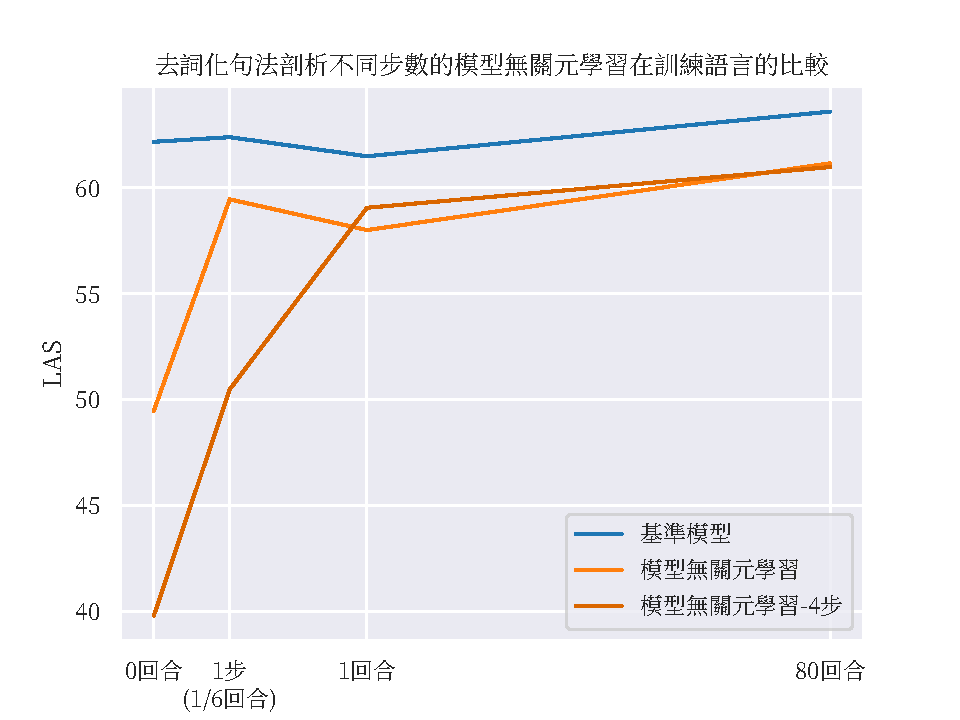
\includegraphics[width=\textwidth]{figs/chapter3/delex/delex_maml_train_langs.pdf}
    \end{subfigure}
    %\vspace{-12pt}
    \begin{subfigure}[b]{0.8\textwidth}
        \centering
        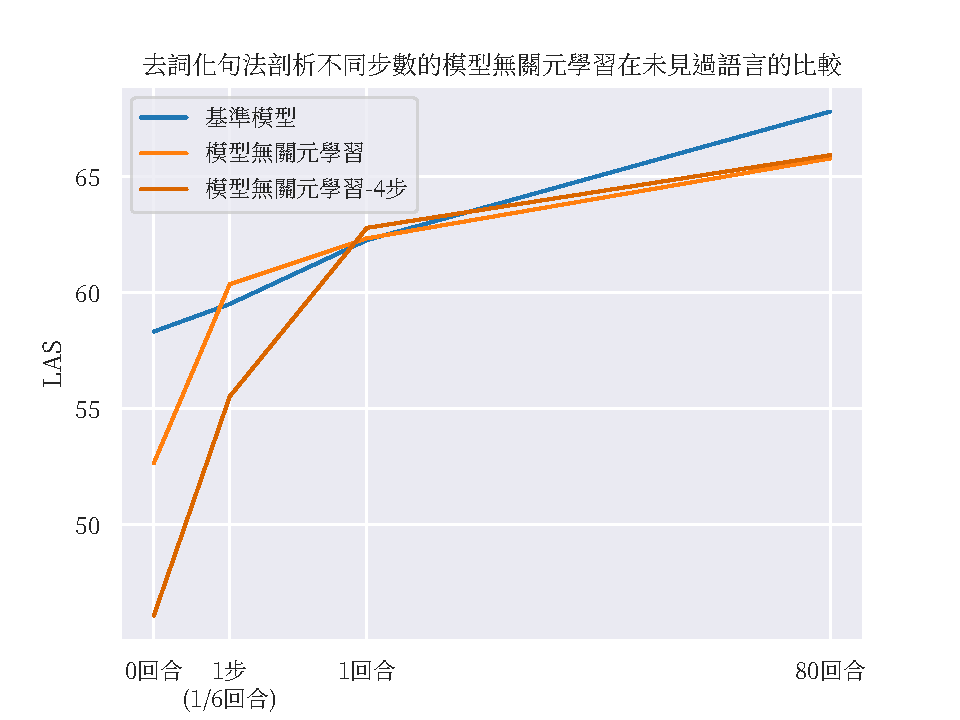
\includegraphics[width=\textwidth]{figs/chapter3/delex/delex_maml_test_langs.pdf}
    \end{subfigure}
    \caption{去詞化分析不同步數的模型無關元學習精細校正後在測試集上的平均表現。}
    \label{fig:delex_avg}
\end{figure}
\begin{figure}[htbp]
    \centering
    \begin{subfigure}[t]{\textwidth}
        \centering
        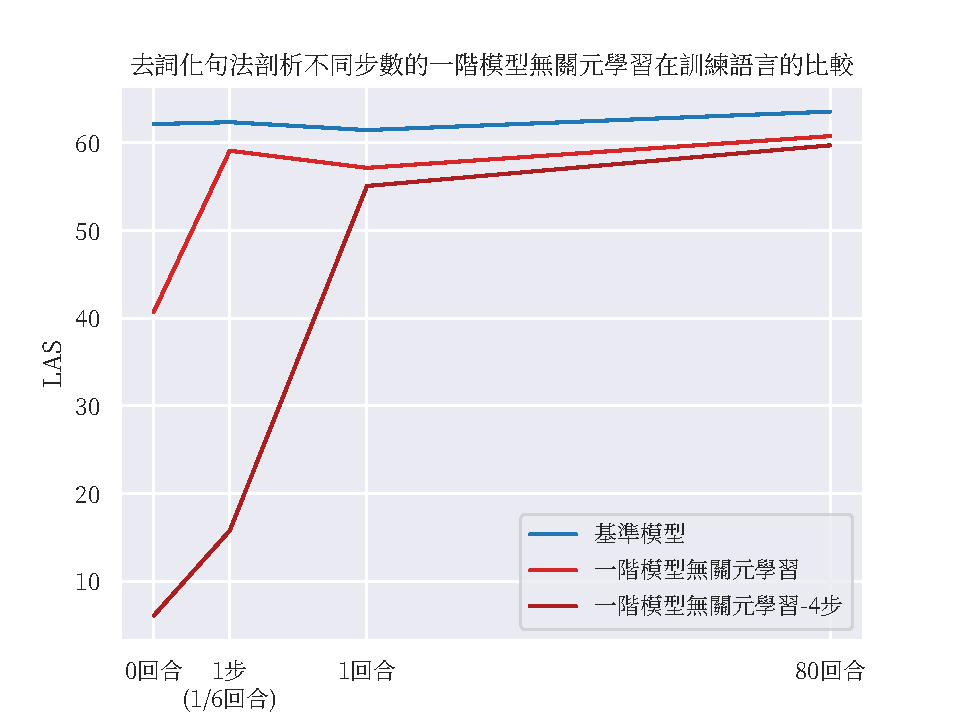
\includegraphics[width=\textwidth]{figs/chapter3/delex/delex_fomaml_train_langs.pdf}
    \end{subfigure}
    \vspace{-12pt}
    \begin{subfigure}[t]{\textwidth}
        \centering
        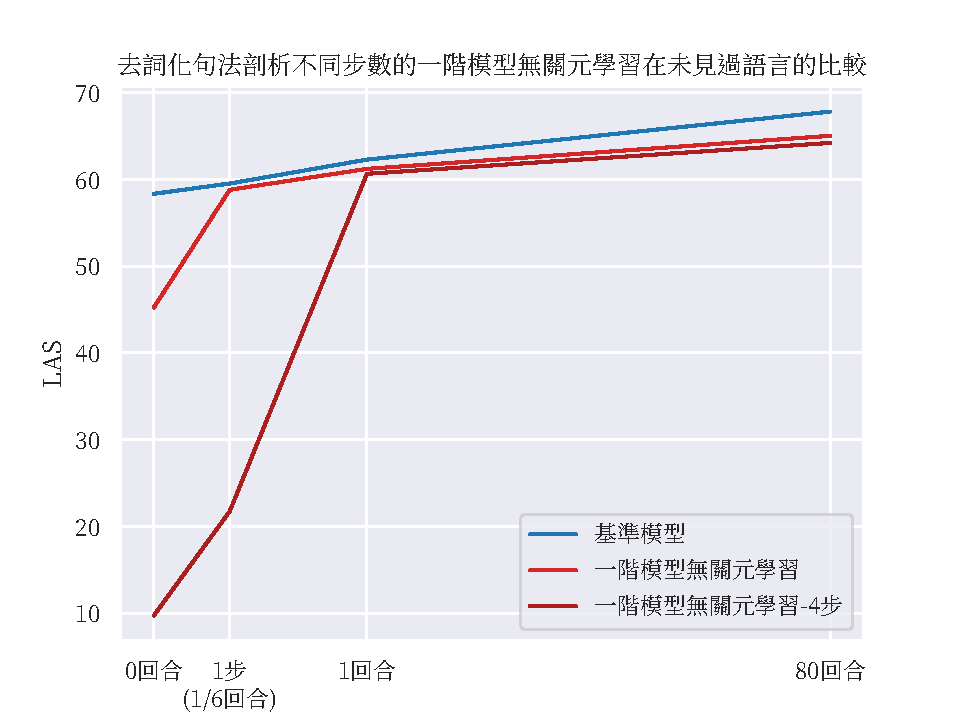
\includegraphics[width=\textwidth]{figs/chapter3/delex/delex_fomaml_test_langs.pdf}
    \end{subfigure}
    \caption{去詞化分析不同步數的一階模型無關元學習精細校正後在測試集上的平均表現。}
    \label{fig:delex_avg}
\end{figure}
\begin{figure}[htbp]
    \centering
    \begin{subfigure}[t]{\textwidth}
        \centering
        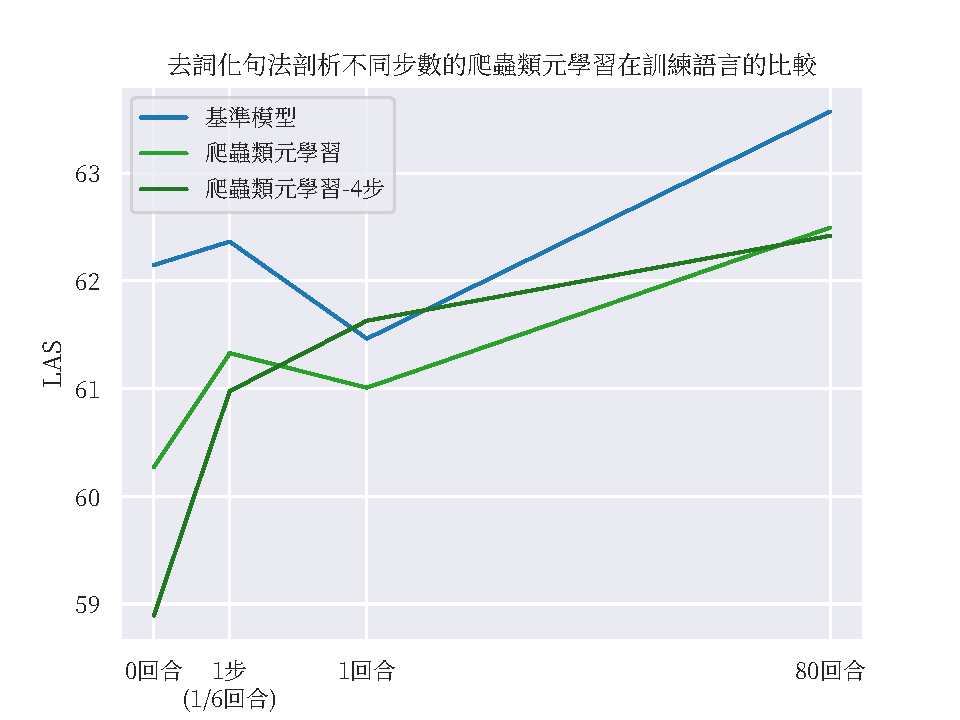
\includegraphics[width=390pt]{figs/chapter3/delex/delex_reptile_train_langs.pdf}
    \end{subfigure}
    \vspace{-12pt}
    \begin{subfigure}[t]{\textwidth}
        \centering
        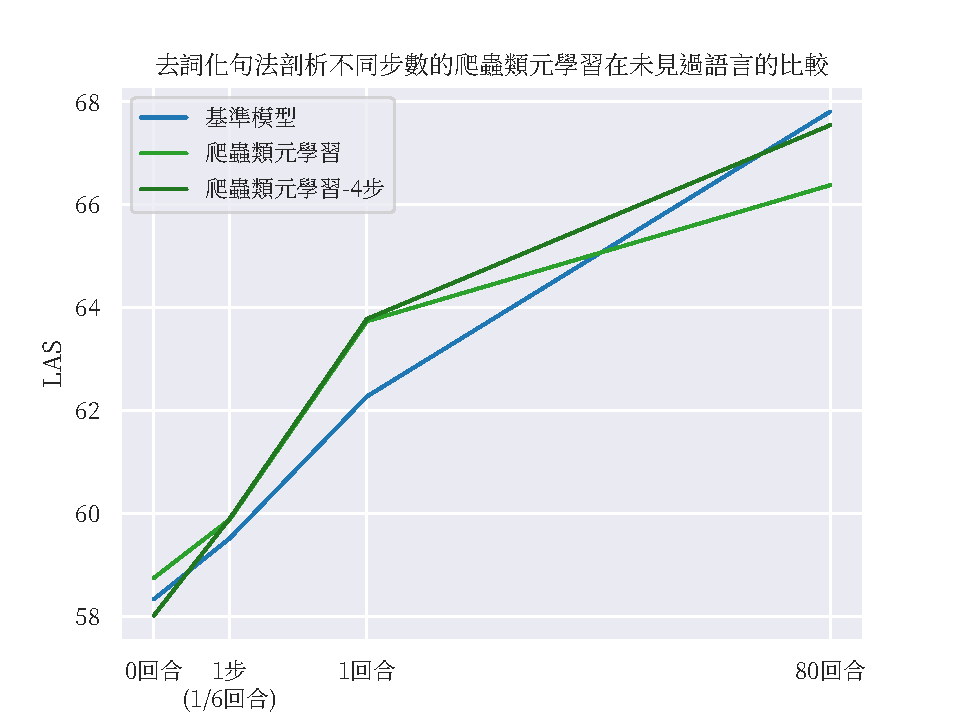
\includegraphics[width=390pt]{figs/chapter3/delex/delex_reptile_test_langs.pdf}
    \end{subfigure}
    \caption{去詞化分析不同步數的爬蟲類元學習精細校正後在測試集上的平均表現。}
    \label{fig:delex_avg}
\end{figure}
\pagebreak
\subsubsection{小模型下各預訓練方法的比較}
\begin{figure}[!htbp]
    \centering
    \begin{subfigure}[t]{0.75\textwidth}
        \centering
        \includegraphics[width=\textwidth]{figs/chapter3/delex/bar_small_zs_train_langs.pdf}
    \end{subfigure}
    \vspace{-12pt}
    \begin{subfigure}[t]{0.75\textwidth}
        \centering
        \includegraphics[width=\textwidth]{figs/chapter3/delex/bar_small_zs_test_langs.pdf}
    \end{subfigure}
    \caption{小模型去詞化分析不同方法在各語言精細校正前的表現。}
    \label{fig:bar_small_zs}
\end{figure}
\begin{figure}[!htbp]
    \centering
    \begin{subfigure}[t]{0.75\textwidth}
        \centering
        \includegraphics[width=\textwidth]{figs/chapter3/delex/bar_small_one_step_train_langs.pdf}
    \end{subfigure}
    \vspace{-12pt}
    \begin{subfigure}[t]{0.75\textwidth}
        \centering
        \includegraphics[width=\textwidth]{figs/chapter3/delex/bar_small_one_step_test_langs.pdf}
    \end{subfigure}
    \caption{小模型去詞化分析不同方法在各語言精細校正一步($\frac{1}{6}$回合)後的表現。}
    \label{fig:bar_small_one_step}
\end{figure}
\begin{figure}[htbp]
    \centering
    \begin{subfigure}[t]{0.8\textwidth}
        \centering
        \includegraphics[width=\textwidth]{figs/chapter3/delex/bar_small_full_epoch_1_train_langs.pdf}
    \end{subfigure}
    \vspace{-12pt}
    \begin{subfigure}[t]{0.8\textwidth}
        \centering
        \includegraphics[width=\textwidth]{figs/chapter3/delex/bar_small_full_epoch_1_test_langs.pdf}
    \end{subfigure}
    \caption{小模型去詞化分析不同方法在各語言精細校正一回合後的表現。}
    \label{fig:bar_small_full_epoch_1}
\end{figure}
\begin{figure}[!htbp]
    \centering
    \begin{subfigure}[t]{0.75\textwidth}
        \centering
        \includegraphics[width=\textwidth]{figs/chapter3/delex/bar_small_full_epoch_80_train_langs.pdf}
    \end{subfigure}
    \vspace{-12pt}
    \begin{subfigure}[t]{0.75\textwidth}
        \centering
        \includegraphics[width=\textwidth]{figs/chapter3/delex/bar_small_full_epoch_80_test_langs.pdf}
    \end{subfigure}
    \caption{小模型去詞化分析不同方法在各語言精細校正八十回合後的表現。}
    \label{fig:bar_small_full_epoch_80}
\end{figure}

%\subsection{限制}
%去詞化分析使用普適詞性標注在多語言句法剖析中,雖然排除了各個語言句法以外性質對句法剖析的影響
\section{多語言依存句法分析(multilingual dependency parsing)}

\subsection{模型架構}

\subsubsection{圖類剖析器 -- 深層雙仿射層注意力網路(Graph-based Parser -- Deep Biaffine Attention)}

2017年由多氏\cite{Dozat2017DeepBA}提出的深層雙仿射層注意力網路(下稱\textbf{雙仿射}),憑藉其簡單的模型架構及強大的實務表現,成爲近年來最常被採用的句法剖析模型。
與其他圖類剖析器一樣,\textbf{雙仿射}的目標為學習邊評分分數:$s(\MWord_{i}, \MWord_{j})$,使得正確句法樹出現的可能性提高。

給定編碼器函數$\MRep\left(\MWord\right) \in \mathbb{R}^{n}$、雙線性矩陣$\mathbf{U}^{(1)} \in \mathbb{R}^{n \times n}$、
線性矩陣$U^{(2)},\ U^{(3)} \in \mathbb{R}^{n} $與偏差$\mathbf{b}$,\textbf{雙仿射}的邊評分函數為:
\begin{equation}
    s(\MWord_{i}, \MWord_{j}) = \MRep(\MWord_{i})^{\top} \mathbf{U}^{(1)} \MRep(\MWord_{j}) + \MRep(\MWord_{i})^{\top} U^{(2)} + \MRep(\MWord_{j})^{\top} U^{(3)} + \mathbf{b}\ .
\end{equation}
上式可分為三部分解釋:$\MRep(\MWord_{i})^{\top} U^{(2)}$代表$w_{i}$接受任何子節點的可能性;$\MRep(\MWord_{j})^{\top} U^{(3)}$代表$w_{j}$接受任何父節點的可能性;
$\MRep(\MWord_{i})^{\top} \mathbf{U}^{(1)} \MRep(\MWord_{j})$則代表$\MWord_{i}$與$\MWord_{j}$之間存在連結(邊)的可能性。

\subsubsection{多語言基於轉換器模型的雙向編碼器表示(multilingual BERT)}

句法剖析的架構中,在大型預訓練語言模型出現以前,編碼器函數$\MRep\left(\MWord\right)$常見的選擇為數層隨機初始化的LSTM或轉換器;
大型預訓練語言模型出現後,以其為編碼器函數的初始訓練參數進行精細校正(fine-tuning)所訓練出的剖析器紛紛取得更好的成績。
多語言的句法剖析在大型預訓練語言模型出現之前較少文獻直接讓各語言共同分享編碼器函數,
真正共享參數的也多為接受詞性標記而非文字的去詞化依存句法剖析(delexicalized dependency parsing),
其原因主要可歸結為多語言模型需要設計統一的記符集(token set)來表示每個語言各異的書寫系統(writing system)產生的文字。
在單語言時可直接用該語言經斷詞後所統計出的常見詞作為記符(token);
單語言的常見詞數目通常設定在10000-40000詞即非常堪用,剩下的低頻詞並不影響模型表現太多;
但多語言模型若不減少任一語言之記符數而直接結合各語言的詞彙做為記符集,此記符集將變得太大,且相近語言無法透過相似的構詞共享參數,
如西班牙文的「學生」一詞``estudiante''與其英文的對應``student''有共同的詞子字串``stud'',上述直接結合的方法便無法讓模型學習到這些共通性。
文獻上已經提出許多解決辦法,以下列舉三項:
\begin{itemize}
    \item 使用語素分割器(morpheme segmenter):利用專家知識構造出基於規則或統計的語素分割器分割語素,並以語素為記符,分割結果符合人類知識,
使相似詞可以正確的共用語素記符向量的參數爲其優點,
惟某些語言可能不存在準確率高的語素分割器,通用性不足。
    \item 使用字符(character)做為記符:優點為不需要某些語言可能沒有的語素分割器,但字符顆粒度過小,單句話的記符數變多,會增加模型處理時間。
    \item 使用次級詞分割(subword tokenization)演算法:次級詞是比詞小但比字符大的記符,
由演算法統計出語言中的詞彙較常獨立出現的子字串(substring)做為新的記符,將詞取代為多個子字串的結合,也可看做是非監督式演算法計算出的語素。
常見的演算法包括字節對編碼(Byte-pair encoding)~\cite{sennrich-etal-2016-neural}、WordPiece \cite{schuster2012japanese}等。
\end{itemize}
其中次級詞雖然分割品質受演算法及訓練語料大小影響良窳不一,但其兼備語素分割器共用子字串與字符不需要人類知識的優點,
因此現行單語言與多語言的大型預訓練語言模型均採用次級詞做為記符來取代原本以詞或字符為單位的表示法。

本研究與目前孔氏提出的多語言句法剖析的最佳單一模型Udify\cite{kondratyuk-straka-2019-75}
一樣採用\textbf{多語言基於轉換器模型的雙向編碼器表示}(下稱$\mathrm{mBERT}$)作為編碼器函數來編碼語料中的衆多語言。

令 $\MRep\left(\MWord\right)$ 為編碼器函數,
$\mathrm{mBERT}\left(\MWord\right)_{i}$為記符$\MWord$通過$\mathrm{mBERT}$第$i$層的輸出,
由於許多文獻\cite{peters-etal-2018-deep,devlin-etal-2019-bert}均指出與其讓下游任務只接受最後一層的輸出,
讓模型在精細校正(fine-tuning)時自由混合幫助較大的輸出層更有助於模型表現,
而特氏也發現\cite{tenney-etal-2019-bert}若交由每個任務自由混合預訓練模型不同層數的輸出,
不同任務所給予的層權重分佈大不相同,其中與句法相關的任務(如詞性標註、句法標註)傾向給予接近輸入的層較大的權重,
而與語意相關的任務則給予接近輸出的層較大的權重,顯示原本只取最後一層的方法恐非最佳策略;
因此這裏採用彼氏(Matthew Peters)提出的層專注機制(layer attention),
給予每一層輸出專注權重,
讓模型決定哪一層的輸出對句法剖析較有幫助:

\begin{equation}
    \MRep\left(\MWord\right) = \alpha \sum_{i=1}^{L} \mathrm{mBERT}\left(\MWord\right)_{i} \cdot \mathrm{softmax} {\left(\mathbf{c}\right)}_{i}
\end{equation}
其中$L$為$\mathrm{mBERT}$的層數(本研究使用\texttt{bert-base-multilingual-cased}版本\footnote{見\url{https://github.com/google-research/bert}},$L=12$),
$\alpha$為可調整的純量,$\mathbf{c} \in \mathbb{R}^{L}$為層專注權重。

為了防止模型過於仰賴特定層的資訊而造成過擬合,這裏採用孔氏提出的\cite{kondratyuk-straka-2019-75}的層丟棄(layer dropout),
在訓練時每個層專注權重$c_{i}$有$p=0.1$的機率被設為$-\infty$,使權重重新分配到其他的層上,
迫使模型整合$\mathrm{mBERT}$全部層輸出的資訊,而非偏重特定某幾層。

\subsubsection{適應器(adapter)}

適應器為雷氏(Sylvestre-Alvise Rebuffi)\cite{rebuffi2018efficient}所提出在影像領域的轉移學習方法,
後由何氏(Neil Houlsby)引進自然語言處理常用的轉換器模型\cite{houlsby2019parameter},
其指出當時自然語言處理的轉移學習方法多半使用大型預訓練轉換器模型進行全模型精細校正在目標任務上,
但何氏認為全模型精細校正需要調整模型中所有的參數,每種任務都會產生一個全新的模型,
太耗費儲存空間與計算資源,且大型預訓練轉換器模型已經含有大量句法語意等任務所需資訊,應不需要變動參數過多;
因此他提出固定原本的大型預訓練轉換器模型參數,但在被固定的模型層中加入具殘差網路性質的適應器,
模型只需為每個任務調整適應器少量的參數,任務間還是共享原本的大型預訓練轉換器模型參數,
而實驗數據也顯示,加入適應器的轉換器模型可以在所需調整的參數量遠低於全模型精細校正下,在目標任務中達成與其相似的表現。
其架構為一前饋層組成的兩層瓶頸網路(一層投射到較小維度,一層投射回原本維度),
再加上殘差連結(residual),置於轉換器中前饋層後、層\XNorm之前的位置,細節可見圖\ref{fig:adapter}。
%其指出學習一通用特徵抽取器(universal feature extractor),
%然後在其後為每個任務接上一個任務專屬模組(task-specific module)做精細校正,
%這樣的方法雖然可以充分利用通用特徵抽取器的精緻特徵一次解決多個任務,但其各自任務的表現通常沒有專精單一任務來得好;
%因此他提出在通用特徵抽取器
\begin{figure}[htbp]
    \centering
    \begin{subfigure}[t]{0.5\textwidth}
        \centering
        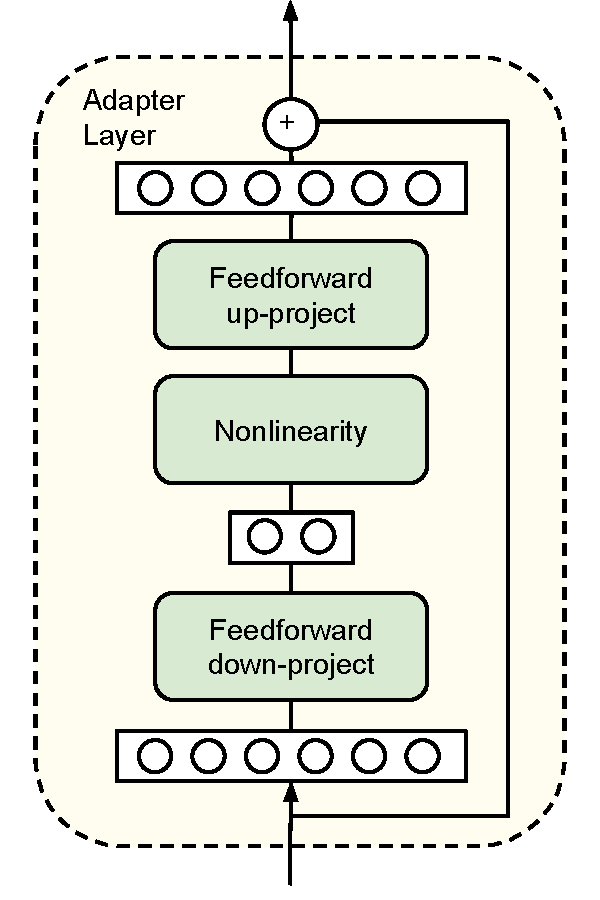
\includegraphics[width=\textwidth]{figs/chapter3/adapters/adapter_arch.pdf}
    \end{subfigure}%
    \begin{subfigure}[t]{0.5\textwidth}
        \centering
        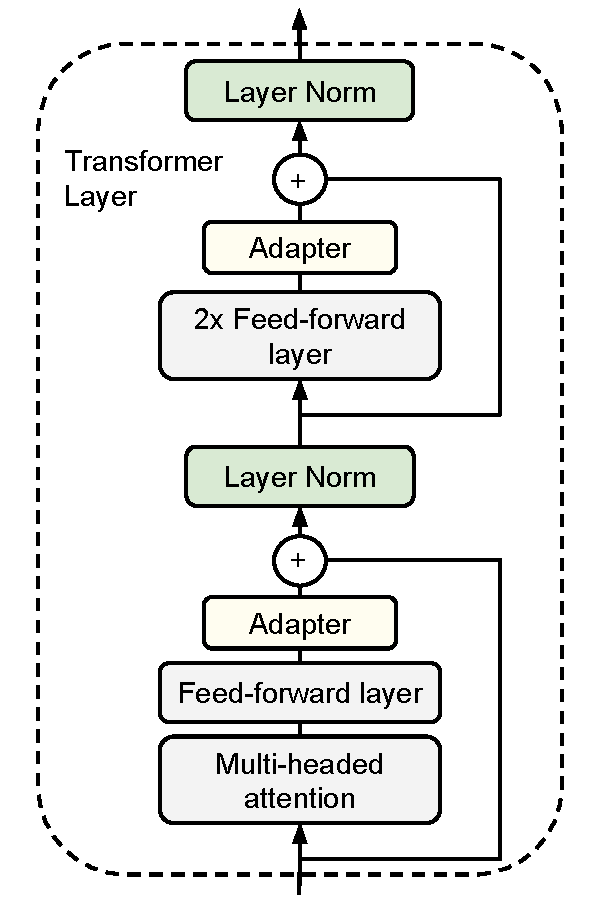
\includegraphics[width=\textwidth]{figs/chapter3/adapters/adapter_insertion.pdf}
        %\caption{加入適應器後的轉換器架構(圖取自\cite{rebuffi2018efficient})。}
    \end{subfigure}
    \caption{\textbf{左側}:適應器架構;\textbf{右側}:加入適應器後的轉換器架構(圖取自\cite{rebuffi2018efficient})。}
    \label{fig:adapter}
\end{figure}
%\input{figs/chapter3/adapters/adapter_ins.tex}

\subsection{實驗設置}

\subsubsection{基準模型與元學習模型共同實驗設置}

本節的實驗設置基於\conll 的實驗設置,但做了些微改變:
我們從\conll 的53種訓練語言(73個訓練句法樹庫)中選取有官方驗證集(development set)的46種訓練語言(66個訓練句法樹庫)作爲訓練語言;見表\ref{tab:training_languages}。
預訓練完成後,我們分別對該模型進行\zeroshot 及\finetune 在預訓練中未見過的語言上。
本節實驗在訓練語言與測試語言的切分與章節\ref{subsec:delex_depparse_setting}去詞化的依存句法剖析設置大致相同,不再贅述,
而訓練方法部分,
在訓練時也均使用正確的斷句、斷詞,
惟測試時爲了與\conll 相比,由於\conll 連句法剖析之前的預處理(斷句、斷詞)也納入整體評分,
但研究重點在句法剖析而非預處理,
因此直接採用StanfordNLP的預處理系統\cite{qi-etal-2018-universal}\footnote{https://github.com/stanfordnlp/stanfordnlp}。

%孔氏\cite{kondratyuk-straka-2019-75}與烏氏\cite{ustun2020udapter}進行多語言訓練的方法,是將全部語言的句法樹庫接在一起、在一個小批次(batch)中混合多個句法樹庫訓練。
%這樣的做法可能會導致資料量大的語言取樣頻率過高;我們的方法則是每次更新從全部語言裡取樣$l$種語言,每種語言取樣$b$個句子,一個批次總共有$b \times l$個句子。
%不同於孔氏與烏氏,這樣的方法防止模型過度對資料充足語言的特性建模,但也可能使得資料不足語言的句子被過度取樣而產生過擬合的現象。

本研究跟隨烏氏的做法,採用適應器模型\finetune $\mathrm{mBERT}$在依存句法剖析任務上。
除了優化器的暖身步數因更改批次大小而跟着更改以外,大部分的超參數都與烏氏的設置一樣;見表\ref{tab:pretrain_hparams}。

其他設置均與章節\ref{subsec:delex_depparse_setting}所述相同。

\subsubsection{元學習實驗設置}

對於\reptile 與\fomaml ,如無特別註明,外迴圈學習率(outer-loop learning rate)與內迴圈學習率(inner loop-learning rate)相同。
\subsubsection{\zeroshot (Zero-shot Transfer)實驗設置}
我們選取CoNLL 2018 Shared Task中只有訓練集而沒有發展集的語言作爲測試語言。

\begin{table}[h!]
\centering
\begin{subtable}[t]{.5\textwidth}
    \begin{tabular}[t]{|l l|}
        \hline
        \textbf{語言} & \textbf{句法樹庫編碼} \\
        \hline
        Afrikaans & af\_afribooms \\
        Ancient Greek & grc\_proiel \\
        Ancient Greek & grc\_perseus \\
        Arabic & ar\_padt \\
        %Armenian & hy\_armtdp \\
        Basque & eu\_bdt \\
        Bulgarian & bg\_btb \\
        %Buryat & bxr\_bdt \\
        Catalan & ca\_ancora \\
        Chinese & zh\_gsd \\
        Croatian & hr\_set \\
        Czech & cs\_cac \\
        Czech & cs\_fictree \\
        Czech & cs\_pdt \\
        Danish & da\_ddt \\
        Dutch & nl\_alpino \\
        Dutch & nl\_lassysmall \\
        English & en\_ewt \\
        English & en\_gum \\
        English & en\_lines \\
        Estonian & et\_edt \\
        Finnish & fi\_ftb \\
        Finnish & fi\_tdt \\
        French & fr\_gsd \\
        French & fr\_sequoia \\
        French & fr\_spoken \\
        Galician & gl\_ctg \\
        Galician & gl\_treegal \\
        German & de\_gsd \\
        Gothic & got\_proiel \\
        Greek & el\_gdt \\
        Hebrew & he\_htb \\
        Hindi & hi\_hdtb \\
        Hungarian & hu\_szeged \\
        Indonesian & id\_gsd \\
        %Irish & ga\_idt \\
        \hline
    \end{tabular}
\end{subtable}%
\begin{subtable}[t]{.5\textwidth}
    \begin{tabular}[t]{|l l|}
        \hline
        \textbf{語言} & \textbf{句法樹庫編碼} \\
        \hline
        Italian & it\_isdt \\
        Italian & it\_postwita \\
        Japanese & ja\_gsd \\
        %Kazakh & kk\_ktb \\
        Korean & ko\_gsd \\
        Korean & ko\_kaist \\
        %Kurmanji & kmr\_mg \\
        Latin & la\_ittb \\
        Latin & la\_proiel \\
        Latin & la\_perseus \\
        Latvian & lv\_lvtb \\
        %North Sami & sme\_giella \\
        Norwegian & no\_bokmaal \\
        Norwegian & no\_nynorsk \\
        Norwegian & no\_nynorsklia \\
        Old Church Slavonic & cu\_proiel \\
        Old French & fro\_srcmf \\
        Persian & fa\_seraji \\
        Polish & pl\_lfg \\
        Polish & pl\_sz \\
        Portuguese & pt\_bosque \\
        Romanian & ro\_rrt \\
        Russian & ru\_syntagrus \\
        Russian & ru\_taiga \\
        Serbian & sr\_set \\
        Slovak & sk\_snk \\
        Slovenian & sl\_ssj \\
        Slovenian & sl\_sst \\
        Spanish & es\_ancora \\
        Swedish & sv\_lines \\
        Swedish & sv\_talbanken \\
        Turkish & tr\_imst \\
        Ukrainian & uk\_iu \\
        %Upper Sorbian & hsb\_ufal \\
        Urdu & ur\_udtb \\
        Uyghur & ug\_udt \\
        Vietnamese & vi\_vtb \\
        \hline
    \end{tabular}
\end{subtable}
\caption{預訓練所使用的訓練句法樹庫/語言。}
\label{tab:training_languages}
\end{table}
\begin{table}[h!]
\centering
\begin{subtable}[t]{.5\textwidth}
    \centering
    \begin{tabular}[t]{|l l|}
        \hline
        \textbf{語言} & \textbf{句法樹庫編碼} \\
        \hline
        Buryat & bxr\_bdt \\
        Kurmanji & kmr\_mg \\
        Upper Sorbian & hsb\_ufal \\
        Armenian & hy\_armtdp \\
        Kazakh & kk\_ktb \\
        Irish & ga\_idt \\
        North Sami & sme\_giella \\
        \hline
    \end{tabular}
    \caption{真實資料不足測試句法樹庫/語言。}
    \label{tab:true_lr_testing_languages}
\end{subtable}%
\begin{subtable}[t]{.5\textwidth}
    \centering
    \begin{tabular}[t]{|l l|}
        \hline
        \textbf{語言} & \textbf{句法樹庫編碼} \\
        \hline
        Wolof & wo\_wtb \\
        Scottish Gaelic & gd\_arcosg \\
        Coptic & cop\_scriptorium \\
        Telugu & te\_mtg \\
        Belarusian & be\_hse \\
        Marathi & mr\_ufal \\
        Maltese & mt\_mudt \\
        Tamil & ta\_ttb \\
        \hline
    \end{tabular}
    \caption{模擬資料不足測試句法樹庫/語言。}
    \label{tab:sim_lr_testing_languages}
\end{subtable}%
\caption{資料不足測試句法樹庫/語言。}
\end{table}
\begin{table}[htbp]
    % \fontsize{8}{10}\selectfont
    \centering
    \begin{subtable}[t]{.4\textwidth}
        \begin{tabular}[t]{@{}lr@{}}
        \toprule
        超參數 & 值 \\
        \midrule
            依存標籤維度         & 256 \\
            依存邊維度           & 768 \\
            丟棄機率            & 0.5 \\
            BERT丟棄機率        & 0.2 \\
            BERT遮蔽機率        & 0.2 \\
            層丟棄機率          & 0.1 \\
            批次大小$b$         & 16 \\
            語言數$l$           & 10 \\
            訓練樣本數/回合        & 64000 \\
            訓練回合數          & 10 \\
            優化器              & Adam \\
            $\beta_1,\beta_2$  & 0.9, 0.99 \\
            權重衰減參數         & 0.01 \\
            基礎學習率          & $1e^{-3}$ \\
            學習率調度器        & ulmfit\_sqrt \\
            學習率暖身步數       & 1231 \\
            最大梯度範數        & 5.0 \\
        \bottomrule
        \end{tabular}
        \caption{
            預訓練超參數。
        }
        \label{tab:pretrain_hparams}
    \end{subtable}
    \begin{subtable}[t]{.4\textwidth}
        \begin{tabular}[t]{@{}lr@{}}
        \toprule
        超參數 & 值 \\
        \midrule
            丟棄機率            & 0.5 \\
            BERT丟棄機率        & 0.2 \\
            BERT遮蔽機率        & 0.2 \\
            層丟棄機率          & 0.1 \\
            批次大小            & 8 \\
            訓練回合數          & 80 \\
            優化器              & Adam \\
            $\beta_1,\beta_2$  & 0.9, 0.99 \\
            權重衰減參數         & 0.01 \\
            基礎學習率          & $5e^{-5}$ \\
            學習率調度器        & slanted\_triangular \\
            學習率暖身步數       & 1(回合)\\
            最大梯度範數        & 5.0 \\
            交叉驗證摺數$k$     & 3   \\
        \bottomrule
        \end{tabular}
        \caption{
            精細校正超參數。
        }
        \label{tab:finetune_hparams}
    \end{subtable}
    \caption{
        模型超參數一覽。
    }
    \label{tab:hparams}
\end{table}

\subsubsection{\finetune (Fine-tuning)實驗設置}
本論文從預訓練完的模型開始對目標語言\finetune 40個回合。其他\finetune 的超參數請見表\ref{tab:finetune_hparams}。

由於選取的測試語言都沒有官方驗證集,在此說明從訓練集中分割出驗證集的方式:
對於訓練集少於100筆資料的語言(有Buryat、Kurmanji、Upper Sorbian、Kazakh、Armenian),以$k$摺交叉驗證(k-fold cross-validation)的方式
得到$k$個模型,並對這$k$個模型做模型集成(model ensemble)。對所有的實驗,我們設$k = 3$;
對於訓練集大於100筆資料的語言(有Irish、North Sami),則隨機切出$\frac{1}{8}$的訓練資料作為驗證資料。

\subsection{實驗結果}
\subsubsection{\zeroshot (Zero-shot Transfer)}
%\begin{figure}[h]
    \centering
    \includegraphics{figs/chapter3/dir_size_las_zs_multi-adapter-crf.pdf}
    \caption{方向性與數據量對基準模型\zeroshot的LAS的影響}
    \label{fig:dir-size-las-zs-multi-adapter-crf}
\end{figure}
基準模型進行\zeroshot 的結果呈現於圖。%\ref{fig:dir-size-las-zs-multi-adapter-crf}。
\iffalse
\begin{table}[!ht]
    \fontsize{8}{10}\selectfont
    \begin{center}
    \setlength{\tabcolsep}{2pt}
    \begin{tabularx}{0.65\textwidth}{@{}l|lcccccccc@{}}
    \toprule
    Setting & Model                             &   bxr   &     kmr   &       hsb &        kk &    hy & ga    & sme   & average \\
    \midrule
    \multirow{ 1}{*}{Baseline} & \sc Stanford   &   13.49 &  \bf   24.15 &     22.97 &     26.25 &     32.70 &  \bf  70.34 &   \bf  70.99 &     27.27 \\
    \hline
    \multirow{ 7}{*}{ZS}
    & $\textsc{Multi}$ & 27.15 & 11.11 & 49.62 & 54.95 & 63.52 & 46.48 & 11.49 & 37.76 \\
    & $\textsc{Fomaml}$ & 26.98 & 11.52 & 48.65 & 53.04 & 62.18 & 46.74 & 11.80 & 37.27 \\
    & $\textsc{Reptile}$ & 27.26 & 11.55 & 49.40 & 53.85 & 62.80 & 47.08 & 11.75 & 37.67 \\
    & $\textsc{Multi\&Reptile}$ & 27.19 & 11.12 & 49.61 & 54.64 & 63.13 & 47.16 & 11.65 & 37.79 \\
    & $\textsc{Multi\&Fomaml}$ & 27.25 & 11.17 & 49.26 & 54.38 & 62.90 & 47.21 & 11.63 & 37.69 \\
    \hline
    \multirow{ 5}{*}{FT} &  \sc Multi                         &     26.37 &     14.86 & \bf 53.98 &     58.63 &     65.81 &     66.39 &     63.63 &     49.95 \\
    & \sc Reptile                       &     27.08 &     14.27 &     52.68 &     58.58 &     66.11 &     66.36 &     63.47 &     49.79 \\
    & $\textsc{Multi}^{\alpha}$              &     24.04 &     15.35 &     48.61 &     51.73 &     54.37 & \bf 67.21 &     63.55 &     46.40 \\
    & $\textsc{Reptile}^{\alpha}$            &     24.69 &     13.72 &     48.96 &     52.14 &     59.93 &     66.98 &     63.50 &     47.13 \\
    & $\textsc{M\&M}$                   & \bf 28.33 & \bf 17.14 &     53.61 & \bf 60.41 & \bf 66.41 &     66.60 & \bf 64.31 & \bf 50.97 \\
    \bottomrule
    \end{tabularx}
    \end{center}
    \caption{\label{table:las_all}
    Zero-shot (ZS) and fine-tuned (FT) test LAS scores of multi-task (\textsc{Multi}), Reptile (\textsc{Reptile}) averaging over seeds, ensemble of two multi-task and reptile models with different seeds ($\textsc{Multi}^{e}$, $\textsc{Reptile}^{e}$),  interpolation of two multi-task and reptile models with different seeds ($\textsc{Multi}^{\alpha}$, $\textsc{Reptile}^{\alpha}$), and interpolation of multi-task and Reptile models with the same random seed ($\textsc{M\&M}$). Our 
    }
\end{table}
\fi
\subsubsection{單語言\finetune (Monolingual Fine-tuning)}

基準模型進行單語言\finetune 的結果呈現於圖\ref{fig:dir-size-las-ft-multi}。從該圖可以發現,句法樹庫的大小幾乎決定了基準模型進行單語言\finetune 在各種語言上的表現。

%\fomaml模型進行單語言\finetune的結果相對於基準模型的進步量呈現於圖\ref{fig:dir-size-las-ft-fomaml-to-multi}。從該圖可以發現,\fomaml主要在資料不足語言表現較基準模型稍佳,而在資料充足語言則差異不大。
模型進行單語言的結果相對於基準模型的進步量呈現於圖\ref{fig:dir-size-las-ft-fomaml-to-multi}。從該圖可以發現,主要在資料不足語言表現較基準模型稍佳,而在資料充足語言則差異不大。

\reptile 模型進行單語言\finetune 的結果相對於基準模型的進步量呈現於圖\ref{fig:dir-size-las-ft-reptile-to-multi}。從該圖可以發現,\reptile 主要在資料不足語言表現較基準模型稍佳,而在資料充足語言則差異不大。

\begin{figure}[h]
    \centering
    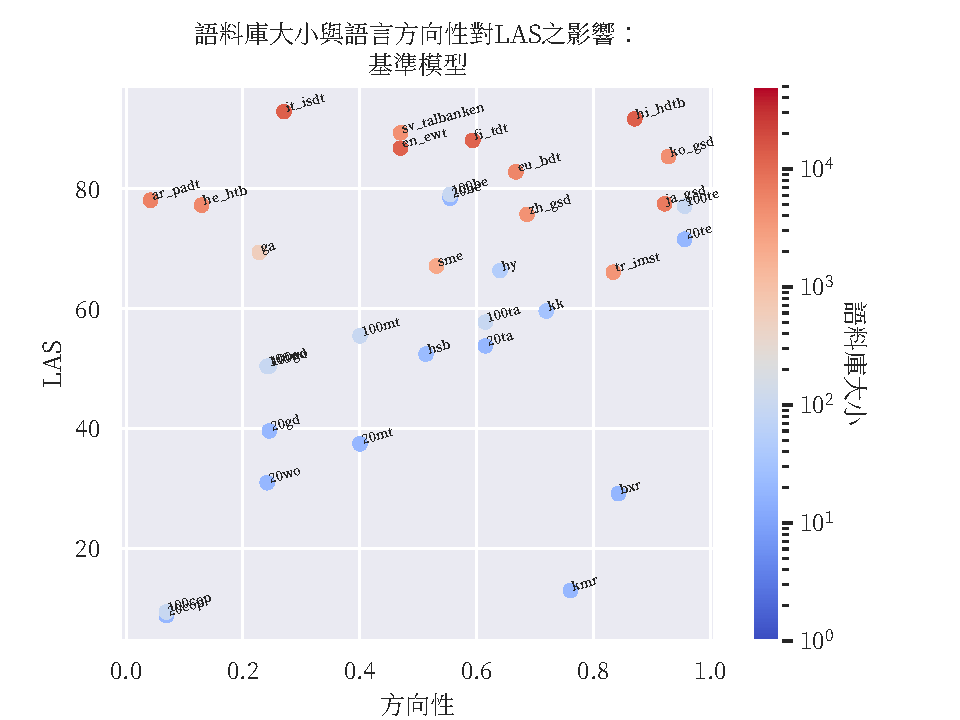
\includegraphics{figs/chapter3/dir_size_las_ft_multi.pdf}
    \caption{方向性與數據量對基準模型進行單語言\finetune後LAS的影響}
    \label{fig:dir-size-las-ft-multi}
\end{figure}

\begin{figure}[h]
    \centering
    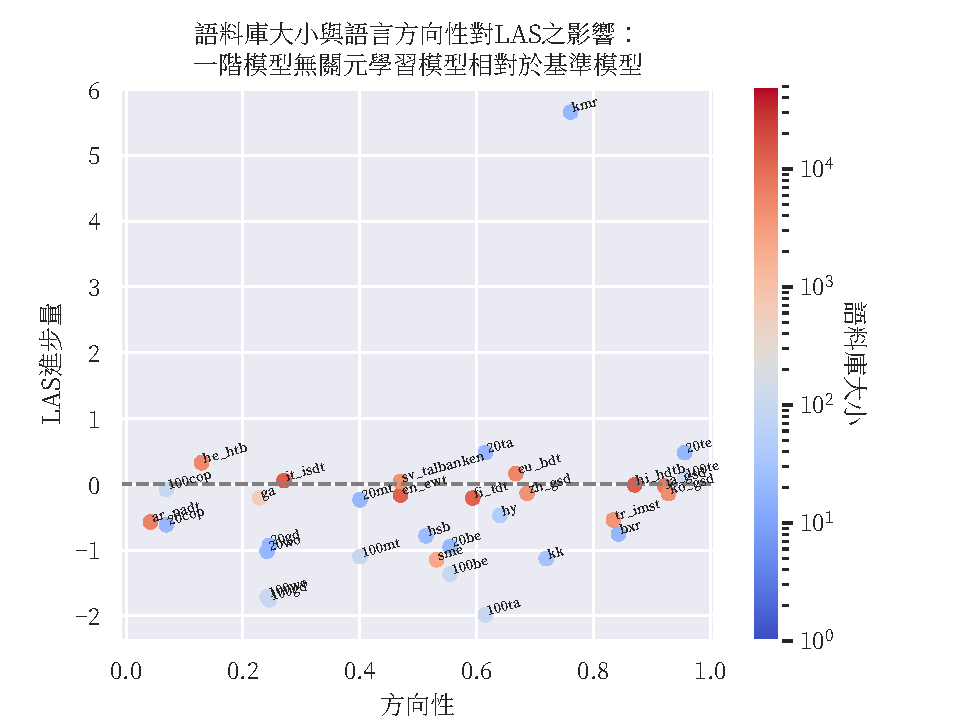
\includegraphics{figs/chapter3/dir_size_las_ft_fomaml-to-multi.pdf}
    \caption{方向性與句法樹庫大小對\fomaml 模型相對於基準模型各自進行單語言\finetune 後LAS之進步量的影響}
    \label{fig:dir-size-las-ft-fomaml-to-multi}
\end{figure}

\begin{figure}[h]
    \centering
    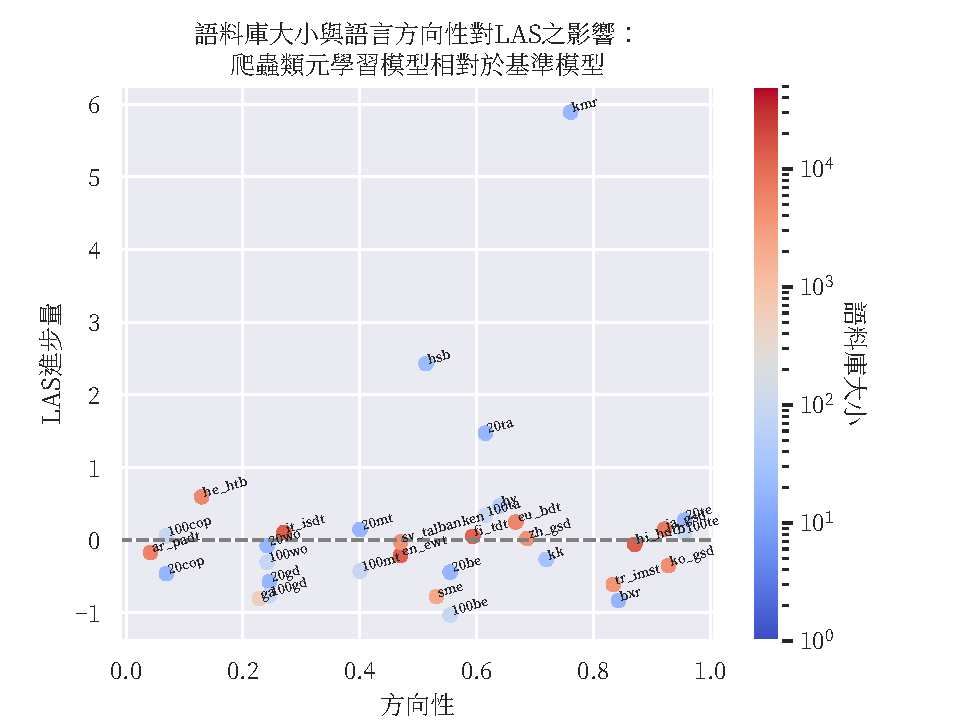
\includegraphics{figs/chapter3/dir_size_las_ft_reptile-to-multi.pdf}
    \caption{方向性與句法樹庫大小對\reptile 模型相對於基準模型各自進行單語言\finetune 後LAS之進步量的影響}
    \label{fig:dir-size-las-ft-reptile-to-multi}
\end{figure}


\chapter{實驗B}
  \section{簡介}
\section{本章總結}

\chapter{實驗C}
  \label{sec:chap5}
\section{簡介}
\section{本章總結}

\chapter{結論與展望}
  \section{研究貢獻與討論}
\section{未來展望}


% this file is encoded in utf-8
% v3.0 (Jun. 11, 2019)

%%% 參考文獻
\newpage
\phantomsection % for hyperref to register this
\addcontentsline{toc}{chapter}{\nameRef}
\renewcommand{\bibname}{\protect\makebox[5cm][s]{\nameRef}}
%  \makebox{} is fragile; need protect
\bibliographystyle{IEEEtran}  % 使用 IEEE Trans 期刊格式
\bibliography{thesis}


%%% 附錄

\newpage
%\phantomsection % for hyperref to register this
%\addcontentsline{toc}{chapter}{\nameAppendix}
\renewcommand\prechaptername{}
\renewcommand\countermapping[1]{#1}
%\renewcommand\tocpostchaptername{}
\renewcommand\postchaptername{}
%\renewcommand{\appendixname}{\protect\makebox[5cm][s]{\nameAppendix}}
\appendix
\chapter{附錄一}
\section{依存句法剖析不同預訓練方法各語言詳細數值}
\label{sec:appendix-bar}
\begin{figure}[htbp]
    \centering
    \begin{subfigure}[t]{0.8\textwidth}
        \centering
        \includegraphics[width=\textwidth]{figs/delex_parsing/barplots/bar_zs_train_langs.pdf}
    \end{subfigure}
    \vspace{-12pt}
    \begin{subfigure}[t]{0.8\textwidth}
        \centering
        \includegraphics[width=\textwidth]{figs/delex_parsing/barplots/bar_zs_test_langs.pdf}
    \end{subfigure}
    \caption{去詞化依存句法剖析不同方法在各語言精細校正前的UAS/LAS長條圖。}
    \label{fig:bar_zs}
\end{figure}
\begin{figure}[htbp]
    \centering
    \begin{subfigure}[t]{0.8\textwidth}
        \centering
        \includegraphics[width=\textwidth]{figs/delex_parsing/barplots/bar_one_step_train_langs.pdf}
    \end{subfigure}
    \vspace{-12pt}
    \begin{subfigure}[t]{0.8\textwidth}
        \centering
        \includegraphics[width=\textwidth]{figs/delex_parsing/barplots/bar_one_step_test_langs.pdf}
    \end{subfigure}
    \caption{去詞化依存句法剖析不同方法在各語言精細校正一步($\frac{1}{6}$回合)後的UAS/LAS長條圖。}
    \label{fig:bar_one_step}
\end{figure}
\begin{figure}[htbp]
    \centering
    \begin{subfigure}[t]{0.8\textwidth}
        \centering
        \includegraphics[width=\textwidth]{figs/delex_parsing/barplots/bar_full_epoch_1_train_langs.pdf}
    \end{subfigure}
    \vspace{-12pt}
    \begin{subfigure}[t]{0.8\textwidth}
        \centering
        \includegraphics[width=\textwidth]{figs/delex_parsing/barplots/bar_full_epoch_1_test_langs.pdf}
    \end{subfigure}
    \caption{去詞化依存句法剖析不同方法在各語言精細校正一回合後的UAS/LAS長條圖。}
    \label{fig:bar_full_epoch_1}
\end{figure}
\begin{figure}[htbp]
    \centering
    \begin{subfigure}[t]{0.8\textwidth}
        \centering
        \includegraphics[width=\textwidth]{figs/delex_parsing/barplots/bar_full_epoch_80_train_langs.pdf}
    \end{subfigure}
    \vspace{-12pt}
    \begin{subfigure}[t]{0.8\textwidth}
        \centering
        \includegraphics[width=\textwidth]{figs/delex_parsing/barplots/bar_full_epoch_80_test_langs.pdf}
    \end{subfigure}
    \caption{去詞化依存句法剖析不同方法在各語言精細校正八十回合後的UAS/LAS長條圖。}
    \label{fig:bar_full_epoch_80}
\end{figure}
\begin{figure}[htbp]
    \centering
    \begin{subfigure}[t]{0.8\textwidth}
        \centering
        \includegraphics[width=\textwidth]{figs/delex_parsing/barplots/bar_small_zs_train_langs.pdf}
    \end{subfigure}
    \vspace{-12pt}
    \begin{subfigure}[t]{0.8\textwidth}
        \centering
        \includegraphics[width=\textwidth]{figs/delex_parsing/barplots/bar_small_zs_test_langs.pdf}
    \end{subfigure}
    \caption{小模型去詞化依存句法剖析不同方法在各語言精細校正前的UAS/LAS長條圖。}
    \label{fig:bar_small_zs}
\end{figure}
\begin{figure}[htbp]
    \centering
    \begin{subfigure}[t]{0.8\textwidth}
        \centering
        \includegraphics[width=\textwidth]{figs/delex_parsing/barplots/bar_small_one_step_train_langs.pdf}
    \end{subfigure}
    \vspace{-12pt}
    \begin{subfigure}[t]{0.8\textwidth}
        \centering
        \includegraphics[width=\textwidth]{figs/delex_parsing/barplots/bar_small_one_step_test_langs.pdf}
    \end{subfigure}
    \caption{小模型去詞化依存句法剖析不同方法在各語言精細校正一步($\frac{1}{6}$回合)後的UAS/LAS長條圖。}
    \label{fig:bar_small_one_step}
\end{figure}
\begin{figure}[htbp]
    \centering
    \begin{subfigure}[t]{0.8\textwidth}
        \centering
        \includegraphics[width=\textwidth]{figs/delex_parsing/barplots/bar_small_full_epoch_1_train_langs.pdf}
    \end{subfigure}
    \vspace{-12pt}
    \begin{subfigure}[t]{0.8\textwidth}
        \centering
        \includegraphics[width=\textwidth]{figs/delex_parsing/barplots/bar_small_full_epoch_1_test_langs.pdf}
    \end{subfigure}
    \caption{小模型去詞化依存句法剖析不同方法在各語言精細校正一回合後的UAS/LAS長條圖。}
    \label{fig:bar_small_full_epoch_1}
\end{figure}
\begin{figure}[htbp]
    \centering
    \begin{subfigure}[t]{0.8\textwidth}
        \centering
        \includegraphics[width=\textwidth]{figs/delex_parsing/barplots/bar_small_full_epoch_80_train_langs.pdf}
    \end{subfigure}
    \vspace{-12pt}
    \begin{subfigure}[t]{0.8\textwidth}
        \centering
        \includegraphics[width=\textwidth]{figs/delex_parsing/barplots/bar_small_full_epoch_80_test_langs.pdf}
    \end{subfigure}
    \caption{小模型去詞化依存句法剖析不同方法在各語言精細校正八十回合後的UAS/LAS長條圖。}
    \label{fig:bar_small_full_epoch_80}
\end{figure}

\begin{figure}[htbp]
    \centering
    \begin{subfigure}[t]{0.8\textwidth}
        \centering
        \includegraphics[width=\textwidth]{figs/lex_parsing/barplots/bar_zs_train_langs.pdf}
    \end{subfigure}
    \vspace{-12pt}
    \begin{subfigure}[t]{0.8\textwidth}
        \centering
        \includegraphics[width=\textwidth]{figs/lex_parsing/barplots/bar_zs_test_langs.pdf}
    \end{subfigure}
    \caption{依存句法剖析不同方法在各語言精細校正前的UAS/LAS長條圖。}
    \label{fig:lex_bar_zs}
\end{figure}
\begin{figure}[htbp]
    \centering
    \begin{subfigure}[t]{0.8\textwidth}
        \centering
        \includegraphics[width=\textwidth]{figs/lex_parsing/barplots/bar_constlr_one_step_train_langs.pdf}
    \end{subfigure}
    \vspace{-12pt}
    \begin{subfigure}[t]{0.8\textwidth}
        \centering
        \includegraphics[width=\textwidth]{figs/lex_parsing/barplots/bar_constlr_one_step_test_langs.pdf}
    \end{subfigure}
    \caption{依存句法剖析不同方法在各語言精細校正一步($\frac{1}{6}$回合)後的UAS/LAS長條圖。}
    \label{fig:lex_bar_one_step}
\end{figure}
\begin{figure}[htbp]
    \centering
    \begin{subfigure}[t]{0.8\textwidth}
        \centering
        \includegraphics[width=\textwidth]{figs/lex_parsing/barplots/bar_constlr_full_epoch_1_train_langs.pdf}
    \end{subfigure}
    \vspace{-12pt}
    \begin{subfigure}[t]{0.8\textwidth}
        \centering
        \includegraphics[width=\textwidth]{figs/lex_parsing/barplots/bar_constlr_full_epoch_1_test_langs.pdf}
    \end{subfigure}
    \caption{依存句法剖析不同方法在各語言精細校正一回合後的UAS/LAS長條圖。}
    \label{fig:lex_bar_full_epoch_1}
\end{figure}
\begin{figure}[htbp]
    \centering
    \begin{subfigure}[t]{0.8\textwidth}
        \centering
        \includegraphics[width=\textwidth]{figs/lex_parsing/barplots/bar_constlr_full_epoch_80_train_langs.pdf}
    \end{subfigure}
    \vspace{-12pt}
    \begin{subfigure}[t]{0.8\textwidth}
        \centering
        \includegraphics[width=\textwidth]{figs/lex_parsing/barplots/bar_constlr_full_epoch_80_test_langs.pdf}
    \end{subfigure}
    \caption{依存句法剖析不同方法在各語言精細校正八十回合後的UAS/LAS長條圖。}
    \label{fig:lex_bar_full_epoch_80}
\end{figure}



%\chapter{\appendixname}
%\section{依存句法剖析不同預訓練方法各語言詳細數值}
\label{sec:appendix-bar}
\begin{figure}[htbp]
    \centering
    \begin{subfigure}[t]{0.8\textwidth}
        \centering
        \includegraphics[width=\textwidth]{figs/delex_parsing/barplots/bar_zs_train_langs.pdf}
    \end{subfigure}
    \vspace{-12pt}
    \begin{subfigure}[t]{0.8\textwidth}
        \centering
        \includegraphics[width=\textwidth]{figs/delex_parsing/barplots/bar_zs_test_langs.pdf}
    \end{subfigure}
    \caption{去詞化依存句法剖析不同方法在各語言精細校正前的UAS/LAS長條圖。}
    \label{fig:bar_zs}
\end{figure}
\begin{figure}[htbp]
    \centering
    \begin{subfigure}[t]{0.8\textwidth}
        \centering
        \includegraphics[width=\textwidth]{figs/delex_parsing/barplots/bar_one_step_train_langs.pdf}
    \end{subfigure}
    \vspace{-12pt}
    \begin{subfigure}[t]{0.8\textwidth}
        \centering
        \includegraphics[width=\textwidth]{figs/delex_parsing/barplots/bar_one_step_test_langs.pdf}
    \end{subfigure}
    \caption{去詞化依存句法剖析不同方法在各語言精細校正一步($\frac{1}{6}$回合)後的UAS/LAS長條圖。}
    \label{fig:bar_one_step}
\end{figure}
\begin{figure}[htbp]
    \centering
    \begin{subfigure}[t]{0.8\textwidth}
        \centering
        \includegraphics[width=\textwidth]{figs/delex_parsing/barplots/bar_full_epoch_1_train_langs.pdf}
    \end{subfigure}
    \vspace{-12pt}
    \begin{subfigure}[t]{0.8\textwidth}
        \centering
        \includegraphics[width=\textwidth]{figs/delex_parsing/barplots/bar_full_epoch_1_test_langs.pdf}
    \end{subfigure}
    \caption{去詞化依存句法剖析不同方法在各語言精細校正一回合後的UAS/LAS長條圖。}
    \label{fig:bar_full_epoch_1}
\end{figure}
\begin{figure}[htbp]
    \centering
    \begin{subfigure}[t]{0.8\textwidth}
        \centering
        \includegraphics[width=\textwidth]{figs/delex_parsing/barplots/bar_full_epoch_80_train_langs.pdf}
    \end{subfigure}
    \vspace{-12pt}
    \begin{subfigure}[t]{0.8\textwidth}
        \centering
        \includegraphics[width=\textwidth]{figs/delex_parsing/barplots/bar_full_epoch_80_test_langs.pdf}
    \end{subfigure}
    \caption{去詞化依存句法剖析不同方法在各語言精細校正八十回合後的UAS/LAS長條圖。}
    \label{fig:bar_full_epoch_80}
\end{figure}
\begin{figure}[htbp]
    \centering
    \begin{subfigure}[t]{0.8\textwidth}
        \centering
        \includegraphics[width=\textwidth]{figs/delex_parsing/barplots/bar_small_zs_train_langs.pdf}
    \end{subfigure}
    \vspace{-12pt}
    \begin{subfigure}[t]{0.8\textwidth}
        \centering
        \includegraphics[width=\textwidth]{figs/delex_parsing/barplots/bar_small_zs_test_langs.pdf}
    \end{subfigure}
    \caption{小模型去詞化依存句法剖析不同方法在各語言精細校正前的UAS/LAS長條圖。}
    \label{fig:bar_small_zs}
\end{figure}
\begin{figure}[htbp]
    \centering
    \begin{subfigure}[t]{0.8\textwidth}
        \centering
        \includegraphics[width=\textwidth]{figs/delex_parsing/barplots/bar_small_one_step_train_langs.pdf}
    \end{subfigure}
    \vspace{-12pt}
    \begin{subfigure}[t]{0.8\textwidth}
        \centering
        \includegraphics[width=\textwidth]{figs/delex_parsing/barplots/bar_small_one_step_test_langs.pdf}
    \end{subfigure}
    \caption{小模型去詞化依存句法剖析不同方法在各語言精細校正一步($\frac{1}{6}$回合)後的UAS/LAS長條圖。}
    \label{fig:bar_small_one_step}
\end{figure}
\begin{figure}[htbp]
    \centering
    \begin{subfigure}[t]{0.8\textwidth}
        \centering
        \includegraphics[width=\textwidth]{figs/delex_parsing/barplots/bar_small_full_epoch_1_train_langs.pdf}
    \end{subfigure}
    \vspace{-12pt}
    \begin{subfigure}[t]{0.8\textwidth}
        \centering
        \includegraphics[width=\textwidth]{figs/delex_parsing/barplots/bar_small_full_epoch_1_test_langs.pdf}
    \end{subfigure}
    \caption{小模型去詞化依存句法剖析不同方法在各語言精細校正一回合後的UAS/LAS長條圖。}
    \label{fig:bar_small_full_epoch_1}
\end{figure}
\begin{figure}[htbp]
    \centering
    \begin{subfigure}[t]{0.8\textwidth}
        \centering
        \includegraphics[width=\textwidth]{figs/delex_parsing/barplots/bar_small_full_epoch_80_train_langs.pdf}
    \end{subfigure}
    \vspace{-12pt}
    \begin{subfigure}[t]{0.8\textwidth}
        \centering
        \includegraphics[width=\textwidth]{figs/delex_parsing/barplots/bar_small_full_epoch_80_test_langs.pdf}
    \end{subfigure}
    \caption{小模型去詞化依存句法剖析不同方法在各語言精細校正八十回合後的UAS/LAS長條圖。}
    \label{fig:bar_small_full_epoch_80}
\end{figure}

\begin{figure}[htbp]
    \centering
    \begin{subfigure}[t]{0.8\textwidth}
        \centering
        \includegraphics[width=\textwidth]{figs/lex_parsing/barplots/bar_zs_train_langs.pdf}
    \end{subfigure}
    \vspace{-12pt}
    \begin{subfigure}[t]{0.8\textwidth}
        \centering
        \includegraphics[width=\textwidth]{figs/lex_parsing/barplots/bar_zs_test_langs.pdf}
    \end{subfigure}
    \caption{依存句法剖析不同方法在各語言精細校正前的UAS/LAS長條圖。}
    \label{fig:lex_bar_zs}
\end{figure}
\begin{figure}[htbp]
    \centering
    \begin{subfigure}[t]{0.8\textwidth}
        \centering
        \includegraphics[width=\textwidth]{figs/lex_parsing/barplots/bar_constlr_one_step_train_langs.pdf}
    \end{subfigure}
    \vspace{-12pt}
    \begin{subfigure}[t]{0.8\textwidth}
        \centering
        \includegraphics[width=\textwidth]{figs/lex_parsing/barplots/bar_constlr_one_step_test_langs.pdf}
    \end{subfigure}
    \caption{依存句法剖析不同方法在各語言精細校正一步($\frac{1}{6}$回合)後的UAS/LAS長條圖。}
    \label{fig:lex_bar_one_step}
\end{figure}
\begin{figure}[htbp]
    \centering
    \begin{subfigure}[t]{0.8\textwidth}
        \centering
        \includegraphics[width=\textwidth]{figs/lex_parsing/barplots/bar_constlr_full_epoch_1_train_langs.pdf}
    \end{subfigure}
    \vspace{-12pt}
    \begin{subfigure}[t]{0.8\textwidth}
        \centering
        \includegraphics[width=\textwidth]{figs/lex_parsing/barplots/bar_constlr_full_epoch_1_test_langs.pdf}
    \end{subfigure}
    \caption{依存句法剖析不同方法在各語言精細校正一回合後的UAS/LAS長條圖。}
    \label{fig:lex_bar_full_epoch_1}
\end{figure}
\begin{figure}[htbp]
    \centering
    \begin{subfigure}[t]{0.8\textwidth}
        \centering
        \includegraphics[width=\textwidth]{figs/lex_parsing/barplots/bar_constlr_full_epoch_80_train_langs.pdf}
    \end{subfigure}
    \vspace{-12pt}
    \begin{subfigure}[t]{0.8\textwidth}
        \centering
        \includegraphics[width=\textwidth]{figs/lex_parsing/barplots/bar_constlr_full_epoch_80_test_langs.pdf}
    \end{subfigure}
    \caption{依存句法剖析不同方法在各語言精細校正八十回合後的UAS/LAS長條圖。}
    \label{fig:lex_bar_full_epoch_80}
\end{figure}



%%% 自傳
%\newpage
%\chapter*{\protect\makebox[5cm][s]{\nameVita}} % \makebox{} is fragile; need protect
%\phantomsection % for hyperref to register this
%\addcontentsline{toc}{chapter}{\nameVita}
%\input{my_vita.tex}



\clearpage % to make sure all CJK characters are processed
\end{CJK}  %%% ZZZ %%%
\end{document} 
 
